\documentclass[UTF8,a4paper,12pt]{ctexbook} 

\usepackage{graphicx}%学习插入图
\usepackage{verbatim}%学习注释多行
\usepackage{booktabs}%表格
\usepackage{geometry}%图片
\usepackage{amsmath}
\usepackage{amssymb}
\usepackage{listings}%代码
\usepackage{xcolor}  %颜色
\usepackage{enumitem}%列表格式
\setenumerate[1]{itemsep=0pt,partopsep=0pt,parsep=\parskip,topsep=5pt}
\setitemize[1]{itemsep=0pt,partopsep=0pt,parsep=\parskip,topsep=5pt}
\setdescription{itemsep=0pt,partopsep=0pt,parsep=\parskip,topsep=5pt}
\usepackage{tcolorbox}
\usepackage{algorithm}  %format of the algorithm
\usepackage{algorithmic}%format of the algorithm
\usepackage{multirow}   %multirow for format of table
\usepackage{tabularx} 	%表格排版格式控制
\usepackage{array}	%表格排版格式控制
\usepackage{hyperref} %超链接 \url{URL}
\usepackage{tikz}
\usepackage{dirtree}

\CTEXsetup[format+={\flushleft}]{section}

%%%% 设置图片目录
\graphicspath{{figure/}}

%%%% 段落首行缩进两个字 %%%%
\makeatletter
\let\@afterindentfalse\@afterindenttrue
\@afterindenttrue
\makeatother
\setlength{\parindent}{2em}  %中文缩进两个汉字位

%%%% 下面的命令重定义页面边距,使其符合中文刊物习惯 %%%%
\addtolength{\topmargin}{-54pt}
\setlength{\oddsidemargin}{0.63cm}  % 3.17cm - 1 inch
\setlength{\evensidemargin}{\oddsidemargin}
\setlength{\textwidth}{14.66cm}
\setlength{\textheight}{24.00cm}    % 24.62

%%%% 下面的命令设置行间距与段落间距 %%%%
\linespread{1.0}
\setlength{\parskip}{0.5\baselineskip}
\geometry{left=1.6cm,right=1.8cm,top=2cm,bottom=1.7cm} %设置文章宽度
\pagestyle{plain} 		  %设置页面布局

%代码效果定义
\definecolor{mygreen}{rgb}{0,0.6,0}
\definecolor{mygray}{rgb}{0.5,0.5,0.5}
\definecolor{mymauve}{rgb}{0.58,0,0.82}
\lstset{ %
	backgroundcolor=\color{white},   % choose the background color
	basicstyle=\footnotesize\ttfamily,      % size of fonts used for the code
	%stringstyle=\color{codepurple},
	%basicstyle=\footnotesize,
	%breakatwhitespace=false,         
	%breaklines=true,                 
	%captionpos=b,                    
	%keepspaces=true,                 
	%numbers=left,                    
	%numbersep=5pt,                  
	%showspaces=false,                
	%showstringspaces=false,
	%showtabs=false,        
	columns=fixed,
	breaklines=true,                 % automatic line breaking only at whitespace
	captionpos=b,                    % sets the caption-position to bottom
	tabsize=4,
	commentstyle=\color{mygreen},    % comment style
	escapeinside={\%*}{*)},          % if you want to add LaTeX within your code
	keywordstyle=\color{blue},       % keyword style
	stringstyle=\color{mymauve}\ttfamily,     % string literal style
	frame=L,
	xleftmargin = .04\textwidth,
	rulesepcolor=\color{red!20!green!20!blue!20},
	% identifierstyle=\color{red},
	escapeinside=``,
	language=c++,
}
 \author{\kaishu 郑华}
 \title{\heiti A·I笔记}
 
\begin{document}          %正文排版开始
 	\maketitle

\chapter{基础概念}
	\section{是什么}
		\begin{figure}[H]
			\centering
			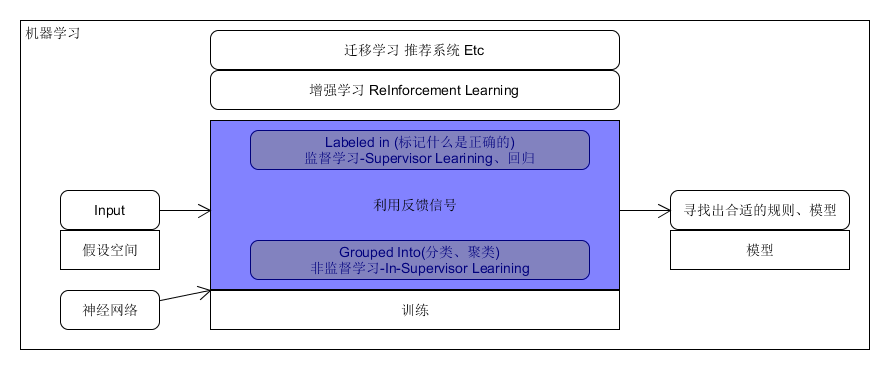
\includegraphics[width=\linewidth]{Basic_001}
			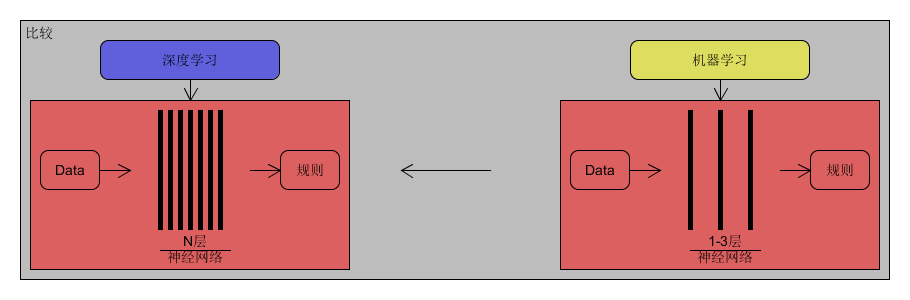
\includegraphics[width=\linewidth]{Basic_002}
		\end{figure}
		
		利用机器学习,人们输入的是数据和从这些数据中预期得到的答案,系统输出的是\textbf{规则}。这些规则随后可应用于新的数据,并使计算机自主生成答案。
		
		机器学习的技术定义:在预先定义好的可能性空间中(数据不同表示-预处理),利用\textbf{反馈信号}的指引来寻找输入数据的有用表示。
		
		机器学习从学习的种类一般分为3种:无监督学习、监督学习、强化学习。
		
		监督学习:每一个样本都有明确的标签(Right Answer),最后总结出这些训练样本向量与标签的映射关系。
		
		无监督学习:在没有标签的情况下尝试找出其内部蕴含关系的一种挖掘工作,常见的如分类、聚合。
		
		强化学习:本质是解决 decision making 问题,即\textbf{自动进行决策},并且可以做连续决策。
	
		\subsection{无监督学习}
			\paragraph{聚类 clustering}
			
		
		\subsection{监督学习}
			\paragraph{分类 classifing}
		
		
			\paragraph{回归 regression}
				通过70\% 的数据训练出规则,通过30\%剩下的数据进行回归测试拟合。	
				
				加入设计的线性关系类似于 $ y = f(x) = wx + b$, 则训练函数类似于
				
				$$ Loss = \sum_{i=1}^{n}|wx_i + b - y_i|$$		
		
		
		\subsection{迁移学习}
			专注于存储已有问题的解决模型,并\textbf{将其利用在其他不同但相关问题上}。比如说,用来辨识汽车的知识(或者是模型)也可以被用来提升识别卡车的能力。
		
		\subsection{强化学习}
			\url{https://blog.csdn.net/j754379117/article/details/83037799}
			
			\url{https://www.jianshu.com/p/5ceca53aff0b}
			
			
			\textbf{强调如何基于环境而行动,以取得最大化的预期利益}。\textit{其灵感来源于心理学中的行为主义理论,即有机体如何在环境给予的奖励或惩罚的刺激下,逐步形成对刺激的预期,产生能获得最大利益的习惯性行为。}
			
			本质是解决 decision making 问题,即\textbf{自动进行决策},并且可以做连续决策。
			
			强化学习最早可以追溯到\textbf{巴甫洛夫的条件反射实验},它从动物行为研究和优化控制两个领域独立发展,最终经Bellman之手将其抽象为\textbf{马尔可夫决策过程} (Markov Decision Process,MDP).
			
			它主要包含四个元素,\textit{agent,环境状态,行动,奖励}, 强化学习的目标就是\textbf{获得最多的累计奖励}。
			
			
			让我们以小孩学习走路来做个形象的\textbf{例子}:
			
			小孩想要走路,但在这之前,他需要先站起来,站起来之后还要保持平衡,接下来还要先迈出一条腿,是左腿还是右腿,迈出一步后还要迈出下一步。
			
			小孩就是 \textbf{agent},他试图通过采取\textbf{行动}(即行走)来适应\textbf{环境}(行走的表面),并且从一个\textbf{状态转变}到另一个状态(即他走的每一步),当他完成任务的子任务(即走了几步)时,孩子得到\textbf{奖励}(给巧克力吃),并且当他不能走路时,就不会给巧克力。
			
			\paragraph{要素}
				几大元素分别是:
				
				\begin{itemize}
					\item \textbf{Agent}  ,输入通常是状态State,输出通常是策略Policy
					\item \textbf{Action} ,就是从一点走到下一点 {A -> B, C -> D, etc},动作空间。比如小人玩游戏,只有上下左右可移动,那Actions就是上、下、左、右。
					\item \textbf{States} ,就是节点 {A, B, C, D, E, F},就是Agent 的输入
					\item \textbf{Reward} ,就是边上的 cost,进入某个状态时,能带来正奖励或者负奖励。
					\item \textbf{Policy} ,就是完成任务的整条路径 {A -> C -> F}
					\item \textbf{Environment} ,接收action,返回state和reward。
				\end{itemize}
				
				\begin{figure}[H]
					\centering
					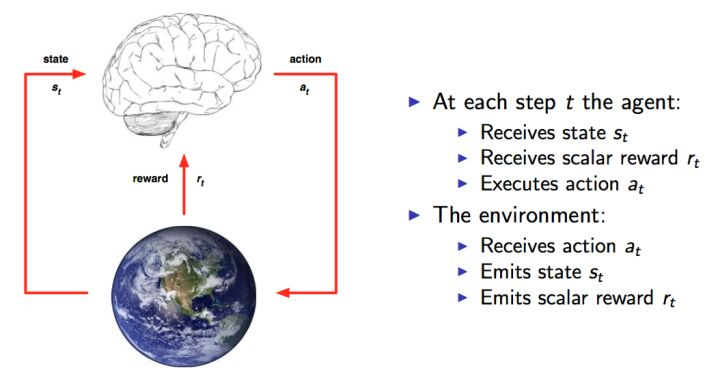
\includegraphics[width=\linewidth]{RL_Basic}
					\caption{强化学习示意}
				\end{figure}
				
				首先通过动作$a_t$与环境$env$进行交互,在动作$a_t$和环境$env$的作用下,Agent 会产生新的状态$s_t$,同时环境会给出一个\textbf{立即回报}$r_t$。
				
				\textit{如此循环下去},智能体与环境进行不断地交互从而产生很多数据。强化学习算法\textbf{利用产生的数据修改自身的动作策略},再与环境交互,产生新的数据,并利用新的数据进一步改善自身的行为,经过数次迭代学习后,智能体能最终地学到完成相应任务的最优动作\textit{(最优策略)}。
				
			\paragraph{分类}
				从强化学习的几个元素的角度划分的话,方法主要有下面几类:
				
				\begin{itemize}
					\item \textbf{Policy based}, 关注点是找到最优策略。
					\item \textbf{Value based}, 关注点是找到最优奖励总和。
					\item \textbf{Action based}, 关注点是每一步的最优行动。
				\end{itemize}
			
			
			\paragraph{特点}
				强化学习所解决的问题的特点:
				\begin{itemize}[itemindent = 1em]
					\item 智能体和环境之间不断进行交互
					\item 搜索和试错
					\item 延迟奖励(当前所做的动作可能很多步之后才会产生相应的结果)
				\end{itemize}
			
				收敛条件或目标:
				\begin{itemize}[itemindent = 1em]
					\item 获取更多的累积奖励
					\item 获得更可靠的估计
				\end{itemize}
			
			
			\paragraph{与其他机器学习的区别}
				\subparagraph{和监督式学习的区别}
					监督式学习就好比你在学习的时候,有一个导师在旁边指点,他知道怎么是对的怎么是错的.
					
					强化学习会\textbf{在没有任何标签的情况下},通过先尝试做出一些行为得到一个结果,通过这个结果是对还是错的反馈,调整之前的行为,就这样不断的调整,算法能够学习到在什么样的情况下选择什么样的行为可以得到最好的结果。
					
					就好比你有一只还没有训练好的小狗,每当它把屋子弄乱后,就减少美味食物的数量(惩罚),每次表现不错时,就加倍美味食物的数量(奖励),那么小狗最终会学到一个知识,就是把客厅弄乱是不好的行为。
					
					\textbf{两种学习方式}\underline{都会学习出输入到输出的一个映射},监督式学习出的是\textbf{之间的关系},\textit{可以告诉算法什么样的输入对应着什么样的输出},强化学习出的是\textbf{给机器的反馈 reward function},\textit{即用来判断这个行为是好是坏}。
					
					\underline{强化学习}的\textbf{结果反馈有延时},有时候可能需要走了很多步以后才知道以前的某一步的选择是好还是坏,而\underline{监督学习}做了比较坏的选择会\textbf{立刻反馈给算法}。
					
					\underline{强化学习}面对的\textbf{输入总是在变化},每当算法做出一个行为,它影响下一次决策的输入,而\underline{监督学习}的输入是\textbf{独立同分布的}。
					
					通过强化学习,一个 agent 可以\textbf{在探索和开发(exploration and exploitation)之间做权衡,并且选择一个最大的回报}。 
					\verb|exploration| 会尝试很多不同的事情,看它们是否比以前尝试过的更好。 
					
					\verb|exploitation| 会尝试过去经验中最有效的行为。
					
					一般的监督学习算法不考虑这种平衡,就只是是 exploitative。
					
					
				\subparagraph{和非监督式学习的区别}
					非监督式不是学习输入到输出的映射,而是\textbf{模式}。例如在向用户推荐新闻文章的任务中,非监督式会找到用户先前已经阅读过类似的文章并向他们推荐其一.
					
					强化学习将通过向用户先推荐少量的新闻,并不断获得来自用户的\textbf{反馈},最后构建用户可能会喜欢的文章的“知识图”。
				
				
				\subparagraph{DQN:Deep-Q-Network}
					深度强化学习全称是 Deep Reinforcement Learning(DRL),其所带来的推理能力 是智能的一个关键特征衡量,真正的让机器有了自我学习、自我思考的能力。
					
					深度强化学习(Deep Reinforcement Learning,DRL)本质上属于\textit{采用神经网络作为值函数估计器的一类方法,其主要优势在于它能够利用深度神经网络对状态特征进行自动抽取,避免了人工 定义状态特征带来的不准确性,使得Agent能够在更原始的状态上进行学习}。
				
	
	\section{视频游戏的AI史}
		\url{https://www.gameres.com/853687.html}
		
		\subsection{Fine State Machine}
		
		\subsection{Monte Calor Search Tree}
		
		\subsection{Behavioral Decision Trees}
		

\chapter{练习环境框架}

	\section{Keras}

	\section{Tensorflow}
	
	\section{PyTorch}
		
		
		
\chapter{监督学习}



\chapter{非监督学习}


\chapter{迁移学习}


\chapter{强化学习-D·Silver}
	\section{参考}
		知乎专栏:\url{https://zhuanlan.zhihu.com/p/25498081}
		
		博客:\url{https://www.cnblogs.com/jinxulin/p/3517377.html}
		
		Towards Data: \url{https://towardsdatascience.com/understanding-markov-decision-processes-b5862c192ddb}
		
		通过例子了解强化学习:\url{http://www.sohu.com/a/228536039_129720} + \\ \url{https://www.freecodecamp.org/news/diving-deeper-into-reinforcement-learning-with-q-learning-c18d0db58efe/}
		
		\begin{figure}[H]
			\centering
			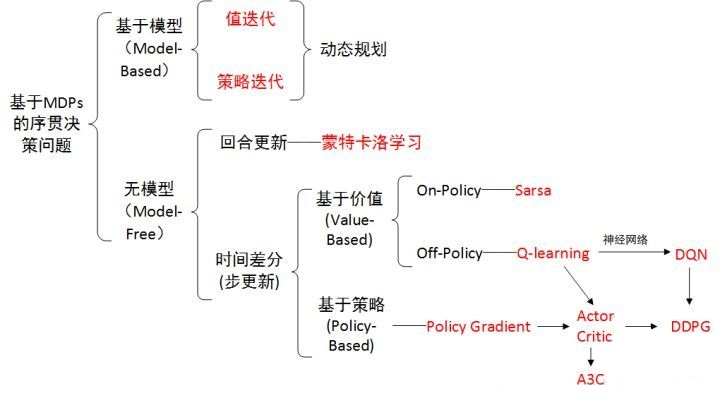
\includegraphics[width=.9\linewidth]{MDPs}
		\end{figure}
		
		
	\section{基本概念}
		\subsection{ModelFree 与 ModelBased}
			model-free是指agent对环境不了解, model-based指agent对环境了解。
				
	
		\subsection{Policy-Based 与  Value-Based}
			\begin{figure}[H]
				\centering
				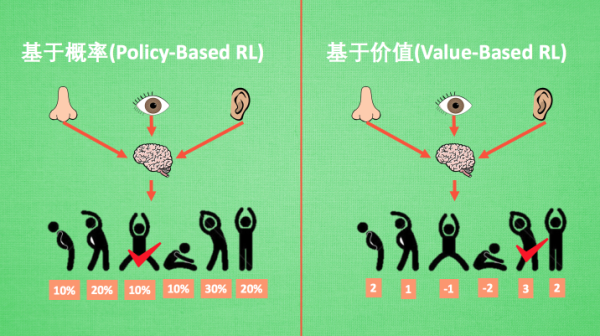
\includegraphics[width=.8\linewidth]{PolicyWithValue}
			\end{figure}
			
			基于概率的话,有几率选到概率比较小的action. 基于价值的话,永远选value最大的动作。另外基于价值的无法在连续动作过程中实现。
		
			在基于概率这边, 有 Policy Gradients, 在基于价值这边有 Q learning, Sarsa 等. 而且我们还能结合这两类方法的优势之处, 创造更牛逼的一种方法, 叫做 Actor-Critic, actor 会基于概率做出动作, 而 critic 会对做出的动作给出动作的价值, 这样就在原有的 policy gradients 上加速了学习过程.
			
		\subsection{OnPolicy  与 OffPolicy}
			\begin{figure}[H]
				\centering
				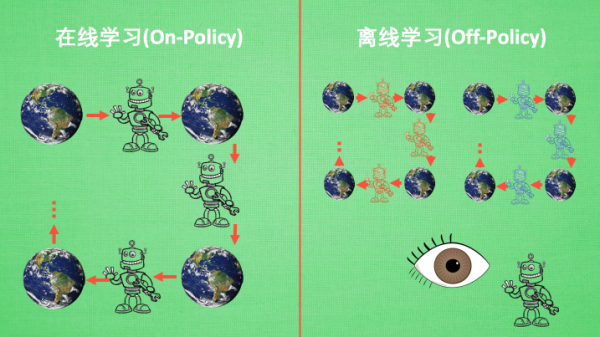
\includegraphics[width=.8\linewidth]{OnOffPolicy}
			\end{figure}

			在线学习, 就是指我必须本人在场, 并且一定是本人边玩边学习。而离线学习是你可以选择自己玩, 也可以选择看着别人玩, 通过看别人玩来学习别人的行为准则。
			
			在线学习有Sarsa, Sarsa lambda, 最典型的离线学习就是 Q learning, Deep-Q-Network.
			
		\subsection{单步更新 与  回合更新}
			\begin{figure}[H]
				\centering
				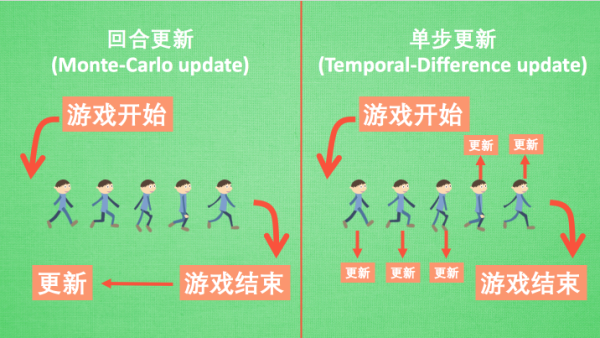
\includegraphics[width=.8\linewidth]{stepWithLoop}
			\end{figure}
		
			回合更新指的是游戏开始后, 我们要等待游戏结束, 然后再总结这一回合中的所有转折点, 再更新我们的行为准则. 而单步更新则是在游戏进行中每一步都在更新, 不用等待游戏的结束, 这样我们就能边玩边学习了.
			
			再来说说方法, Monte-carlo learning 和基础版的 policy gradients 等 都是回合更新制, Qlearning, Sarsa, 升级版的 policy gradients 等都是单步更新制. 因为单步更新更有效率, 所以现在大多方法都是基于单步更新. 
	
		\subsection{强化学习的解法的通用框架}
			有限马尔科夫状态(finite MDP)包含有限的状态集和动作集。大多数强化学习的理论或算法都需要马尔科夫过程的前提限制,但是其思想具有广泛通用性。
		
	\section{MDP-马尔可夫决策}
		\subsection{马尔科夫性质}
			马尔科夫性是指系统的下一个状态$s_{t+1}$仅与当前状态$s_t$有关,而与以前的状态无关。
			
			定义:状态$s_t$是马尔科夫的,当且仅当$P[S_{t+1}|s_t] = P[s_{t+1}|s_1,...,s_t]$。
			
			定义中可以看到,当前状态$s_t$其实是蕴含了所有相关的历史信息$s_1,...,s_t$,一旦当前状态已知,历史信息将会被抛弃。
			
		\subsection{马尔科夫过程}
			马尔科夫性描述的是\textbf{每个状态的性质},但真正有用的是如何描述\textbf{一个状态序列}。数学中用来描述\textbf{随机变量序列}的学科叫\textbf{随机过程}。所谓随机过程就是指随机变量序列。
			
			若随机变量序列中的每个状态都是马尔科夫的则称此随机过程为马尔科夫随机过程。
			
			马尔科夫过程的定义:马尔科夫过程是一个二元组$(S,P)$,且满足:$S$是有限状态集合, $P$是状态转移概率。状态转移概率矩阵为:
			$$
				P = \left[
							\begin{array}{ccc}
								\mathbf{P_{11}} & \cdots & \mathbf{P_{1n}}\\
								
								\vdots & \vdots & \vdots\\
								
								\mathbf{P_{n1}} & \cdots & \mathbf{P_{nn}}\\
							\end{array}
					\right]
			$$
			
			\paragraph{示例}
				一个学生的7种\textbf{状态}{娱乐,课程1,课程2, 课程3,考过,睡觉,论文},每种\textit{状态之间}有一定的\textbf{转换概率}。具体如下图所示。
				
				\begin{figure}[H]
					\centering
					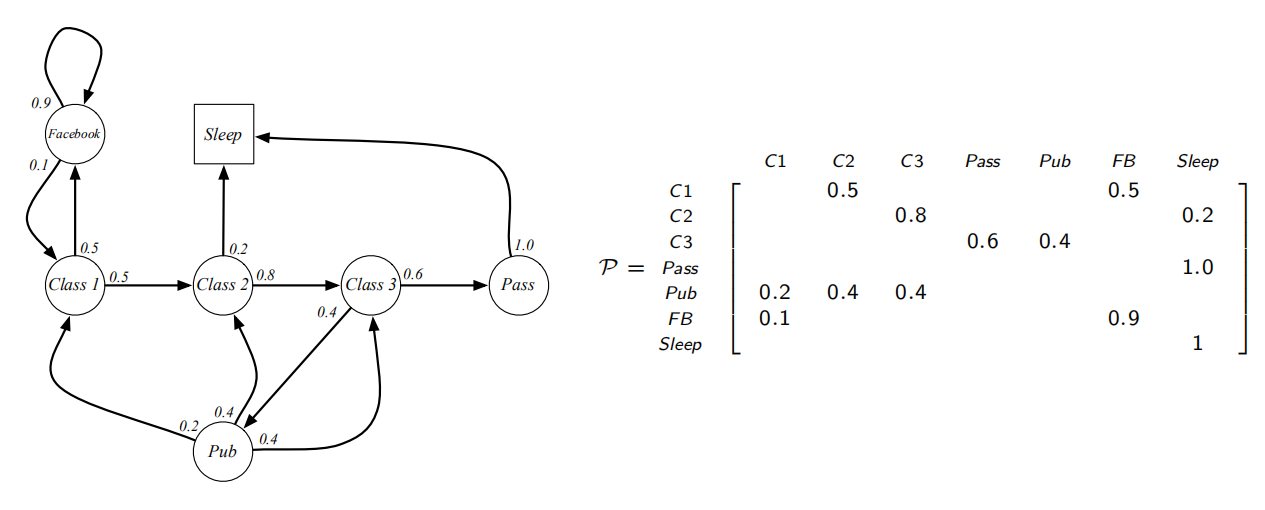
\includegraphics[width=.9\linewidth]{MDP-example}
					\caption{马尔可夫决策示例}
				\end{figure}
				
				以上状态序列称为马尔科夫链。当给定状态转移概率时,从某个状态出发存在多条\textbf{马尔科夫链}。对于游戏或者机器人,马尔科夫过程不足以描述其特点,因为不管是游戏还是机器人,他们都是通过动作与环境进行交互,并从环境中获得奖励,\textbf{而马尔科夫过程中不存在动作和奖励}。\textbf{将动作(策略)和回报考虑在内的马尔科夫过程称为马尔科夫决策过程}。
				
		\subsection{马尔科夫决策过程}
		
			\paragraph{基本组成}
			基本组成:五元组 $M=(S,A,P,\gamma,R)$.
								
			\begin{itemize}[itemindent = 1em]
				\item \textbf{S}: 表示状态集(states),有$s \in S$,$s_i$表示第i步的状态。
				
				\item \textbf{A}: 表示一组动作(actions),有$a \in A$,$a_i$表示第i步的动作,由状态与策略函数$\pi$ 决定。
				
				\item \textbf{P}: 表示状态转移概率。$s$ 表示的是在当前$s \in S$状态下,经过$a \in A$作用后,会转移到的其他状态的\textbf{概率分布情况}。比如,在状态s下执行动作a,转移到s'的概率可以表示为 $p(s'|s,a)$。
				
				\item \textbf{R}: $S \times A->\mathbb{R}$,R是回报函数(reward function)。有些回报函数状态S的函数,可以简化为$R:S->\mathbb{R}$。如果一组$(s,a)$转移到了下个状态$s'$,那么回报函数可记为$r(s'|s, a)$。如果 $(s,a)$ 对应的下个状态s'是唯一的,那么回报函数也可以记为$r(s,a)$。
				
				\textit{回报函数}可以看成是一个映射,关于当前的动作,或者当前环境和当前动作的pair的好不好的一个评价。\textbf{属于立即评价,只考虑当前这一步的好坏}。
				
				\item $\mathbf{\gamma}$ :折现因子:对未来的价值抱有的希望参数,取值在$[0,1]$
			\end{itemize}
			
			
			\paragraph{状态转移策略$\pi(s)$}	
				policy --在当前环境的基础上,引入动作Action,并将环境和动作之间添加一种映射,\textbf{某种环境下最应该做什么动作呢?这个是由policy决定的}。policy的所有可能组成一个policy空间,强化学习的目的,就是在这个巨大的空间中,学习到某一种最优的policy。
			
			
				马尔科夫决策过程的状态转移概率是包含动作的:
				$$ P_{ss1}^a = P[S_{t+1} = s1 | S_t = s, A_t = a]$$
				
				\begin{figure}[H]
					\centering
					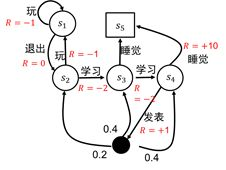
\includegraphics[width=.7\linewidth]{MDP-example2}
					\caption{马尔可夫决策过程示例}
				\end{figure}			
				
				学生有五个状态,状态集为$S = {s_1, s_2, s_3, s_4, s_5}$,动作集为$A={\textit{玩},\textit{退出},\textit{学习},\textit{发论文},\textit{睡觉}}$,在上图中$R$表示\textbf{立即回报}。
				
				强化学习的\textbf{目标}是给定一个马尔科夫决策过程,\textbf{寻找最优策略}。所谓\textit{策略是指状态到动作的映射},策略常用符号$\pi$表示,它是指给定状态$s$时,动作集上的一个分布,即
				
				\begin{equation}
					\pi(a|s) = p[A_t = a_t | S_t = s]
				\end{equation}
				
				策略的定义是用条件概率分布给出的。策略$\pi$在每个状态$s$指定一个动作概率。如果给出的策略$\pi$是确定性的,那么策略$\pi$在每个状态$s$指定一个确定的动作。
				
				例如其中一个学生的策略为$\pi_1(\textit{玩}|s_1) = 0.8$,是指该学生在状态$s_1$时玩的概率为0.8,不玩的概率是0.2,显然这个学生更喜欢玩。
				
				另外一个学生的策略为$\pi_2(\textit{玩}|s_1) = 0.3$,是指该学生在状态[公式]时玩的概率是0.3,显然这个学生不爱玩。依此类推,每学生都有自己的策略。
			
			\paragraph{累积回报$G_t(s)$}	
				和上面的\textit{reward function}对比着看,这一步考虑的是当前环境状态的\textbf{长远优势},也就是\textbf{以当前状态为起点,以后的多个时间点之后的各个状态的reward之和}。如何更好的估计这个值,是几乎所有增强学习问题的解决重点和难点。这个也是如何评定一个policy好坏的标准。
			
				\textbf{强化学习是找到最优的策略,这里的最优是指得到的总回报最大。}
				
				当给定一个策略$\pi$时,就可以计算\textbf{累积回报}了。首先定义\textbf{累积回报}:
				\begin{equation}
					G_t = R_{t+1} + \gamma R_{t+2} + \cdots = \sum_{k=0}^\infty \gamma^k R_{t+k+1}
				\end{equation}
				
				注意:这里某个时间点上的$G_t$,也就是\textbf{期望返回值},是从该时间点往后所有获取的reward序列和.
				
				\verb|discounting rate| $\gamma \in [0,1]$: 决定了未来奖励的当前价值.
				
				\verb|discounting rate| 的含义就是,在当前时间点k步之后的奖励,在当前的价值是未来的$\gamma^{k-1}$倍。当该系数小于1,最终和会收敛,只要奖励序列是有限的。当系数为0,则执行机构是短视的,只顾眼前利益;如果系数大于1,执行机构是远视的,也就是重视长远奖励。
				
				在策略$\pi$下,可以计算累积回报$G_1$,此时$G_1$有多个可能值 。\textbf{由于策略}$\pi$\textbf{是随机的,因此累积回报也是随机的}。\textit{为了评价状态}$s_1$\textit{的价值},我们需要定义一个确定量来描述状态$s_1$的价值,很自然的想法是利用累积回报来衡量状态$s_1$的价值。然而,累积回报$G_1$是个随机变量,不是一个确定值,因此无法进行描述。\textbf{但其期望是个确定值,可以作为\underline{状态值函数}的定义。}
				
			
			\paragraph{状态-价值函数$V_t(s)$}
			
				累积回报$G$是个随机变量,不是一个确定值,因此\textbf{无法评价}状态$s$\textit{的价值}。但其期望是个确定值(\textbf{状态值}$v_\pi$),可以作为评价依据。
			
				当Agent采用策略$\pi$时,累积回报服从一个分布,累积回报在状态$s$处的期望值定义为\textbf{状态-值函数}:
				\begin{equation}
					\begin{aligned}
						v_\pi(s) &= E_\pi \left[\sum_{k=0}^{\infty}\gamma^k R_{t+k+1}|S_t = s \right]	\\
							&= R_s + \gamma \sum_{s' \in S}P_{ss'}v(s') \\
							&= \textit{立即回报} + \textit{未来回报}
					\end{aligned}
				\end{equation}
				
				\verb|-->|状态值函数是与策略$\pi$相对应的,这是因为策略$\pi$决定了累积回报$G$的状态分布.
			
			\paragraph{动作:价值函数$q(a)$}
				把每个action的真实value定义为$q_*(a)$,把每个action在第t个时间步下的估计值定义为$q_t(a)$。
				
				每个action的真实value,是当该动作被选择时所获得的期望reward,在这里,自然想到用最简洁的历史平均reward来表示当前动作的value估计值。假定某个action在t时间前总共被选择了$k_\alpha$次,于是我们的估计值如下式:
			
				$$q_t(a) = \dfrac{R_1 + R_2 + \cdots + R_{k_\alpha}}{t}$$
				
				这个方法叫做sample-average,因为每个动作的estimated value都是依据过往sample reward的平均值进行计算的。当$k_\alpha$等于0,我们可以把定义为一个默认的初始值,当$k_\alpha$趋近无穷,则最终收敛于$q_*(a)$。当然这个estimate的方法不一定是最好的,只是为了说明问题而已。
				
				可以发现,为了算在t时间的action a的value estimation,我们需要t时间之前所有时间该动作的reward记录。随着时间增加,这种计算方式涉及的计算复杂度和存储压力都会增加。
				
				其实这是不必要的,我们完全可以用另一种方式来计算$q_t(a)$。推导如下:
				
				$$\begin{aligned}
				Q_{n+1} &= \frac{1}{n}\sum_{i=1}^{n}R_i \\
				        &= \frac{1}{n}(R_n + \sum_{i=1}^{n-1}R_i) \\
				        &= \frac{1}{n}(R_n + (n-1)\frac{1}{n-1} \sum_{i=1}^{n-1}R_i) \\
				        &= \frac{1}{n}(R_n + (n-1)Q_n) \\
				        &= \frac{1}{n}(R_n + nQ_n-Q_n) \\
				        &= Q_n + \frac{1}{n}(R_n - Q_n)
				\end{aligned}
				$$
				
				用这个形式的迭代公式,只需要保存$q_k(a)$和$k$,再加上一点简单的加减运算,就可以快速得到$q_{k+1}(a)$, 这个形式的写法贯穿于全文。
				
				
				$$ newEstimate \gets oldEstimate + stepSize(target - oldEstimate)$$
				
				$target-oldEstimate$ 是 $estimate$ 的error,乘以stepsize是\textbf{不断地减小这个error,逼近target}。
				
				
			\paragraph{状态-行为:价值函数$q_\pi(s,a)$}
				相应地,状态-行为 \textit{价值函数}为:
				
				\begin{equation}
					\begin{aligned}
					q_\pi(s,a) &= E_\pi \left[\sum_{k=0}^{\infty}\gamma^k R_{t+k+1}|S_t = s, A_t = a \right]\\
							&= R_s^a + \gamma \sum_{s'\in S} P_{ss'}^a\sum_{a'\in A}\pi(a'|s')q_\pi(s', a')
					\end{aligned}
				\end{equation}
				
				因为引入了动作策略,因而在每一个状态下策略$\pi$ 都会有该状态下会发生动作的概率分布空间,而每种动作都可能导致不同的后续状态。具体关联如下所示:
				
				\begin{figure}[H]
					\centering
					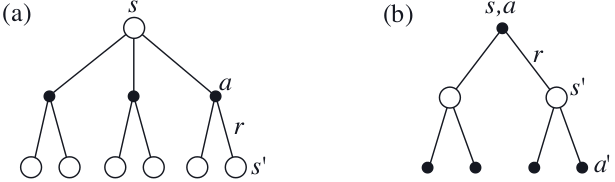
\includegraphics[width=.7\linewidth]{qV}
					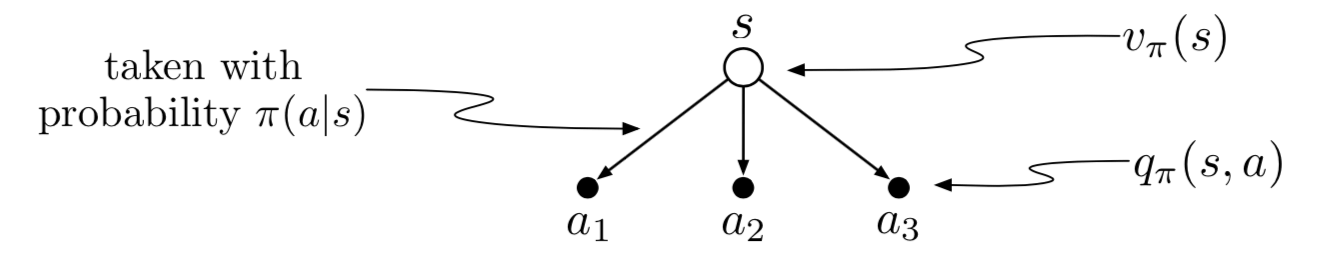
\includegraphics[width=.8\linewidth]{qV01}
					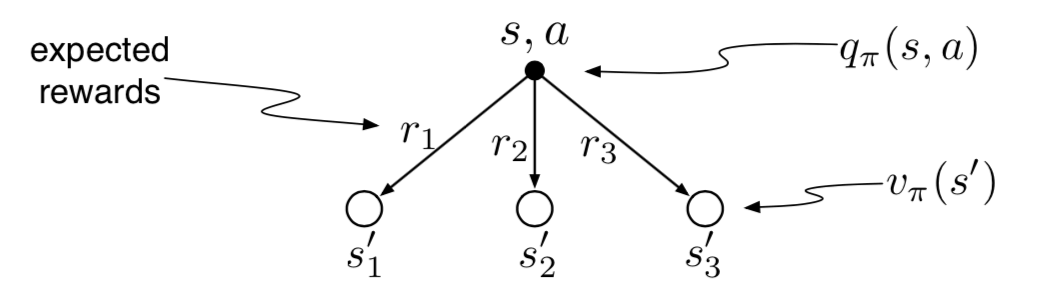
\includegraphics[width=.8\linewidth]{qV02}
					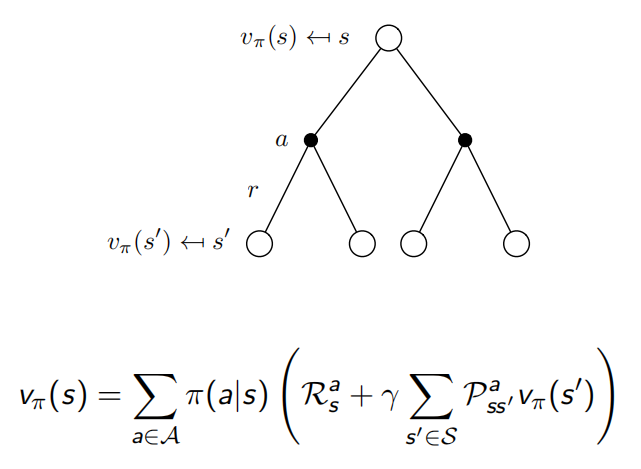
\includegraphics[width=.6\linewidth]{qV03}
					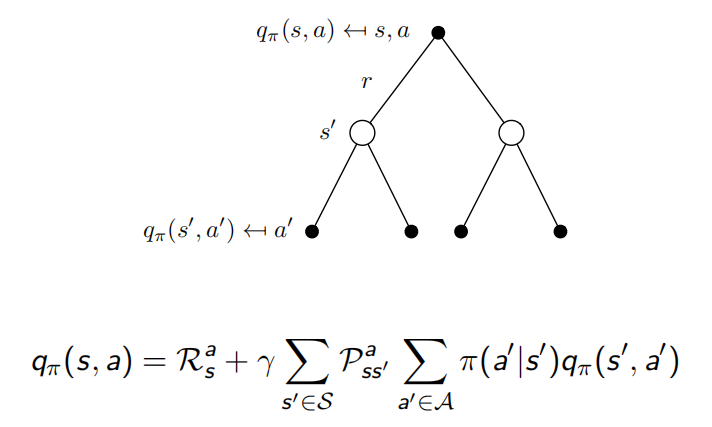
\includegraphics[width=.6\linewidth]{qV04}
					\caption{状态与动作的关联示例}
					\label{q(a,s)}
				\end{figure}
				
				其中空心表示状态,实心表示某状态下可能产生的动作分布。
				
				从状态 $s$ 开始,顶部的根节点,个体可以采取基于其策略 $\pi$ 的任何一组动作,图中显示了三个。 这些动作中的每一个,环境可以响应下一个状态中的其中一个,$s′$ (图中显示两个), 以及奖励 $r$,取决于函数 $p$ 给出的动态。
				
				\begin{figure}[H] 
					\centering
					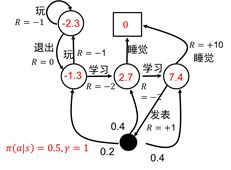
\includegraphics[width=.8\linewidth]{MDP-example3}
					\caption{状态值函数示例}
				\end{figure}		
								
				图中白色圆圈中的数值为该状态下的值函数。即:$v_\pi(s_1) = -2.3, v_\pi(s_2) = -1.3, v_\pi(s_3) = 2.7, v_\pi(s_4) = 7.4, v_\pi(s_5) = 0$			
				
				\verb|-->Notice:|图中,除了pub 这个动作外,其余各状态也可以看成是执行了某动作,但是其通往某状态的概率为1. 既$s \to a \to s'$ 过程中,$a \to s'$ 的概率始终为1,所以不存在其他分支, 因而没有画中间类似于pub 的动作与状态的关联图。	
			
			\paragraph{状态:价值函数与状态-行为:价值函数的贝尔曼方程}
				
				贝尔曼方程对上述图\ref{q(a,s)}中$s \to s'$所有可能性进行平均,通过其发生概率对每个可能性进行加权。 它指出,开始状态的值必须等于预期的\textbf{下一个状态的(衰减)值},加上\textbf{沿途预期的奖励}。
			
				由\textit{状态值函数}的定义式可以得到:
				
				\begin{equation}
					\begin{aligned}
						v(s) &= E[G_t|S_t = s]	\\
							&= E[R_{t+1} + \gamma R_{t+2} + \cdots | S_t = s] \\
							&= E[R_{t+1} + \gamma (R_{t+2} + \gamma R_{t+3} + \cdots)|S_t = s]\\
							&= E[R_{t+1} + \gamma G(t+1)|S_t = s]	\\
							&= E[R_{t+1} + \gamma E_{s_{t+1},\cdots}(G(S_{t+1}))]	\\
							&= E[R_{t+1} + \gamma v(S_{t+1})|S_t = s]	\\
							&= \textit{立即回报} + \textit{未来回报}
					\end{aligned}
				\end{equation}
				
				需要注意的是对哪些变量求期望。
				
				同样我们可以得到状态-动作值函数的贝尔曼方程:
				
				\begin{equation}
					q_\pi(s,a) = E_\pi[R_{t+1} + \gamma q(S_{t+1},A_{t+1})|S_t = s, A_t = a]
				\end{equation}
				
				
			
			\paragraph{最优:价值函数}
				可以通过以下方式精确地定义一个最优策略。价值函数对策略进行部分排序。 如果策略$\pi$所有状态的预期返回值大于或等于策略$\pi'$的值, 则该策略 $\pi$被定义为优于或等于策略 $\pi'$。 换句话说,对所有 $s \in S$, 当且仅当$v_\pi(s)\ge v_{\pi^{^\prime}}(s)$时,$\pi\ge\pi^\prime$ 成立。 总是至少有一个策略优于或等于所有其他策略。这个策略称为 最优策略。 虽然可能有不止一个,我们用 $\pi_*$ 表示所有最优策略。 它们共享同样的状态值函数,称为 最优状态价值函数,表示为 $v_∗$,并定义为
			
				$$ v_*(s) \doteq \max_\pi v_\pi(s) $$
				
			\paragraph{最优动作:价值函数}
				最优策略还具有相同的最优动作价值函数,表示为 $q_∗$,并定义为
				
				$$q_*(s,a) \doteq \max_\pi q_\pi(s,a)$$
				
				对所有 $s \in S$和 $a \in A(s)$. 对于状态—动作对$(s,a)$,此函数给出在状态 $s$ 中执行动作 $a$ 并且此后遵循最优策略的预期返回值。 因此,我们可以用 $v_∗$ 来表示 $q_∗$ ,如下所示:
				
				$$q_*(s,a) = \mathbb{E}\left[R_{t+1}+\gamma v_* (S_{t+1})|S_t=s,A_t=a\right]$$
			
			
			\paragraph{最优BellMan 方程}
				贝尔曼最优方程式表达了这样一个事实,即最优策略下的状态价值必须等于来自该状态的最佳行动的预期收益:
			
				$$\begin{aligned}
				v_*(s) &= \max_{a\in\mathcal{A}(s)} q_{\pi_*}(s,a) \\
				&=\max_a \mathbb{E}_{\pi_*}[G_t|S_t=s,A_t=a] \\
				&=\max_a \mathbb{E}_{\pi_*}[R_{t+1}+\gamma G_{t+1}|S_t=s,A_t=a]  \\
				&=\max_a \mathbb{E}[R_{t+1}+\gamma v_*(S_{t+1})|S_t=s,A_t=a] \\
				&=\max_{a\in \mathcal{A}(s)}\sum_{s^\prime,r} p(s^\prime,r|s,a)[r+\gamma v_*(s^\prime)]
				\end{aligned}$$
						
				最后两个方程是 $v_∗$ 的贝尔曼最优方程的两种形式,$q_∗$ 的贝尔曼最优方程为	
				
				$$
				\begin{aligned}
				q_*(s,a) &= \mathbb{E}\left[R_{t+1}+\gamma\sum_{a^\prime}q_*(S_{t+1,a^\prime})|S_t=s,A_t=a\right] \\
				&=\sum_{s^\prime,r}p(s^\prime,r|s,a)[r+\gamma \sum_{a^\prime}q_*(s^\prime,a^\prime)]
				\end{aligned}$$	
				
				与上述状态-行为 价值函数相似的关联如下所示:
				
				\begin{figure}[H]
					\centering
					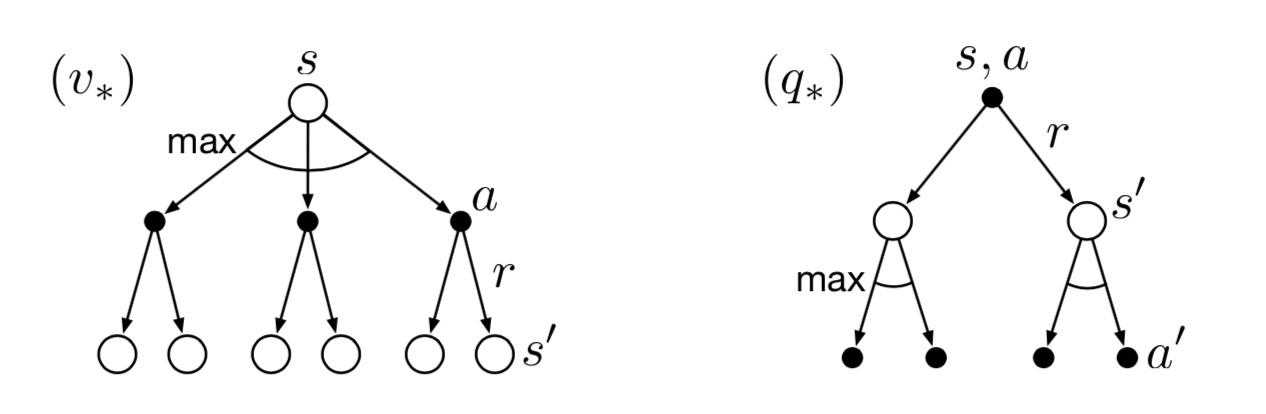
\includegraphics[width=\linewidth]{qVStar}
					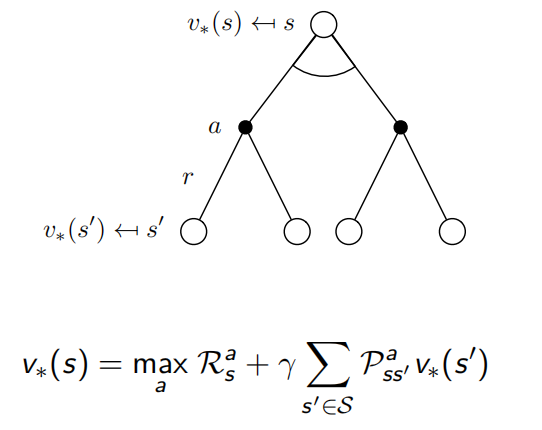
\includegraphics[width=.7\linewidth]{qVStar01}
					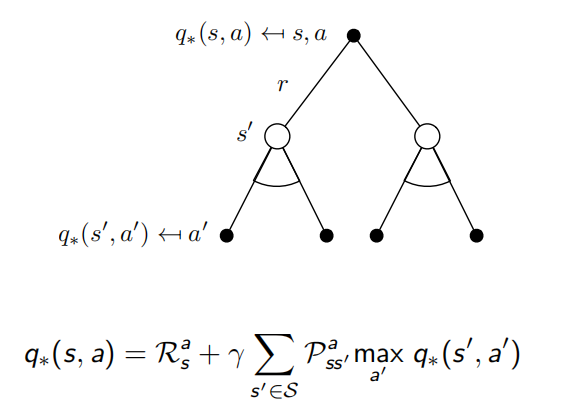
\includegraphics[width=.7\linewidth]{qVStar02}
				\end{figure}
				
				\begin{figure}[H]
					\centering
					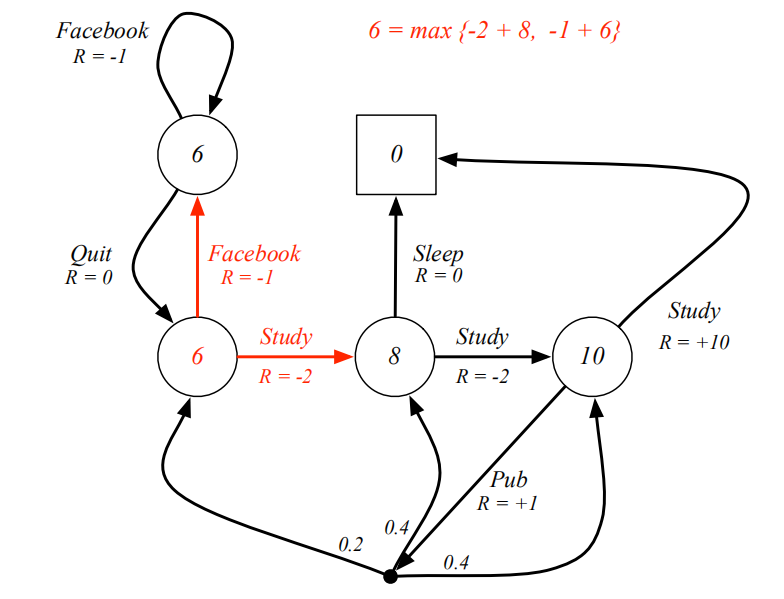
\includegraphics[width=\linewidth]{qVStar03}
				\end{figure}
	
	
		\subsection{总结}
			
			\begin{table}[H]
				\centering
				\caption{MDP 相关概念}
				\begin{tabular}{p{4cm}|p{11.5cm}}
					\toprule
					关键点  &  定义		\\
					\midrule
					状态转移矩阵	&	$ P_{ss'}^a = P[S_{t+1} = s1 | S_t = s, A_t = a]$ 分布	\\
					\hline
					Reward Function	&	$R_s^a = E[R_{t+1}|S_t = s, A_t = a]$  固定,不是随机变量				\\
					\hline
					Policy		&	$\pi(a|s) = P[A_t = a| S_t = s]$ 分布	\\
					\hline
					Return		& $G_t = R_{t+1} + \gamma R_{t+2} + \cdots = \sum_{k=0}^\infty \gamma^k R_{t+k+1}$		\\
					\hline
					state-value function	&	$V_\pi(s) = E_\pi[G_t | S_t = s]$	\\
					\hline
					action-value function 	&	$Q_\pi(s,a) = E_\pi[G_t | S_t = s, A_t = a]$	\\
					\hline
					Expectation Equation \textbf{For Predict}	&	$ \begin{cases}
						v_\pi(s) =  R_s + \gamma \sum_{s' \in S}P_{ss'}v(s')  \textit{     加权平均-下同}	\\
						q_\pi(s,a) = R_s^a + \gamma \sum_{s'\in S} P_{ss'}^a\sum_{a'\in A}\pi(a'|s')q_\pi(s', a')
					\end{cases}$	\\
					\hline
					Optimal Equation \textbf{For Control}&	$ \begin{cases}
											v_*(s) = Max( R_s + \gamma \sum_{s' \in S}P_{ss'}v(s') ) \textit{     加权平均取最大值-下同}	\\
											q_*(s,a) =Max( R_s^a + \gamma \sum_{s'\in S} P_{ss'}^a\sum_{a'\in A}\pi(a'|s')q_*(s', a') )
										\end{cases}$	\\					
					\bottomrule
				\end{tabular}
			\end{table}
		
		
		
		
	\section{Model-Based 动态规划}
		当有了一个可以完美模拟马尔可夫过程的模型之后,\textbf{如何计算最优policies}?。(\textit{注意是policies,表明最优的策略可能不止一个})。
		
		\subsection{prediction-评估一个策略}
			首先考虑给定任意策略$\pi$怎样计算状态值函数$v_\pi$。 这在DP文献中被称作 \textbf{策略评估}、或者Prediction。
		
		\subsection{control-找到最优策略}
			\subsubsection{ - Policy iteration- }
				等若干步迭代 再greedy 更新一次.
				
				计算某个策略价值函数的目的是找到一个更好的策略。假设我们已经确定了一个任意确定性的策略$\pi$价值函数 $v_\pi$。 对于某些状态 $s$ 我们想知道是否应该改变策略来明确的选择一个动作 $a ≠ \pi(s)$。 
				
				我们知道在当前状态 $s$ 遵从当前的策略有多好——>也就是 $v_\pi(s)$——但是改变为一个新的状态会更好还是坏呢? 一种解决这个问题的方法是考虑从状态 s 下选择动作 a,然后遵从现有的策略 $\pi$。
			
				
				\begin{figure}[H]
					\centering
					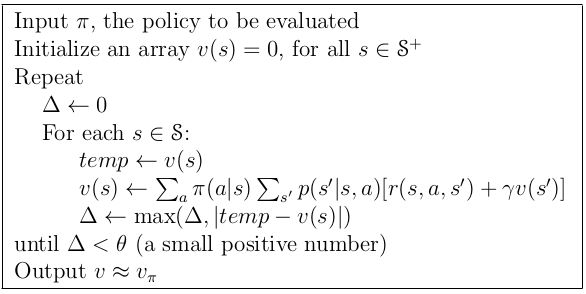
\includegraphics[width=.75\linewidth]{dp00}
				\end{figure}
			

				一旦策略 $\pi$,已经用 $v_\pi$ 提升为更好的策略 $\pi'$, 我们可以计算 $v_\pi'$ 再次提升策略得到更好的策略 $\pi''$。 我们可以得到一系列单调提升的策略和价值函数:
				
				$$ \pi_0 \overset{E}{\rightarrow} v_{\pi_0} \overset{I}{\rightarrow} \pi_1 \overset{E}{\rightarrow} v_{\pi_1} \overset{I}{\rightarrow} \pi_2 \overset{E}{\rightarrow} \cdots \overset{I}{\rightarrow} \pi_* \overset{E}{\rightarrow} v_{*} $$
				
			
				\begin{figure}[H]
					\centering
					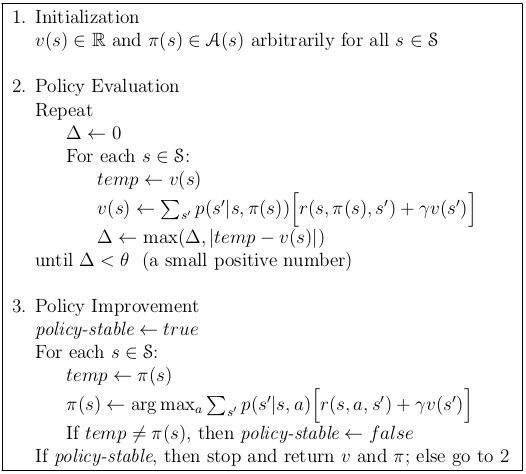
\includegraphics[width=.75\linewidth]{dp01}
				\end{figure}			
			
			\subsubsection{- Value iteration- }
				每一步迭代 都greedy 更新一次
				
				\begin{figure}[H]
					\centering
					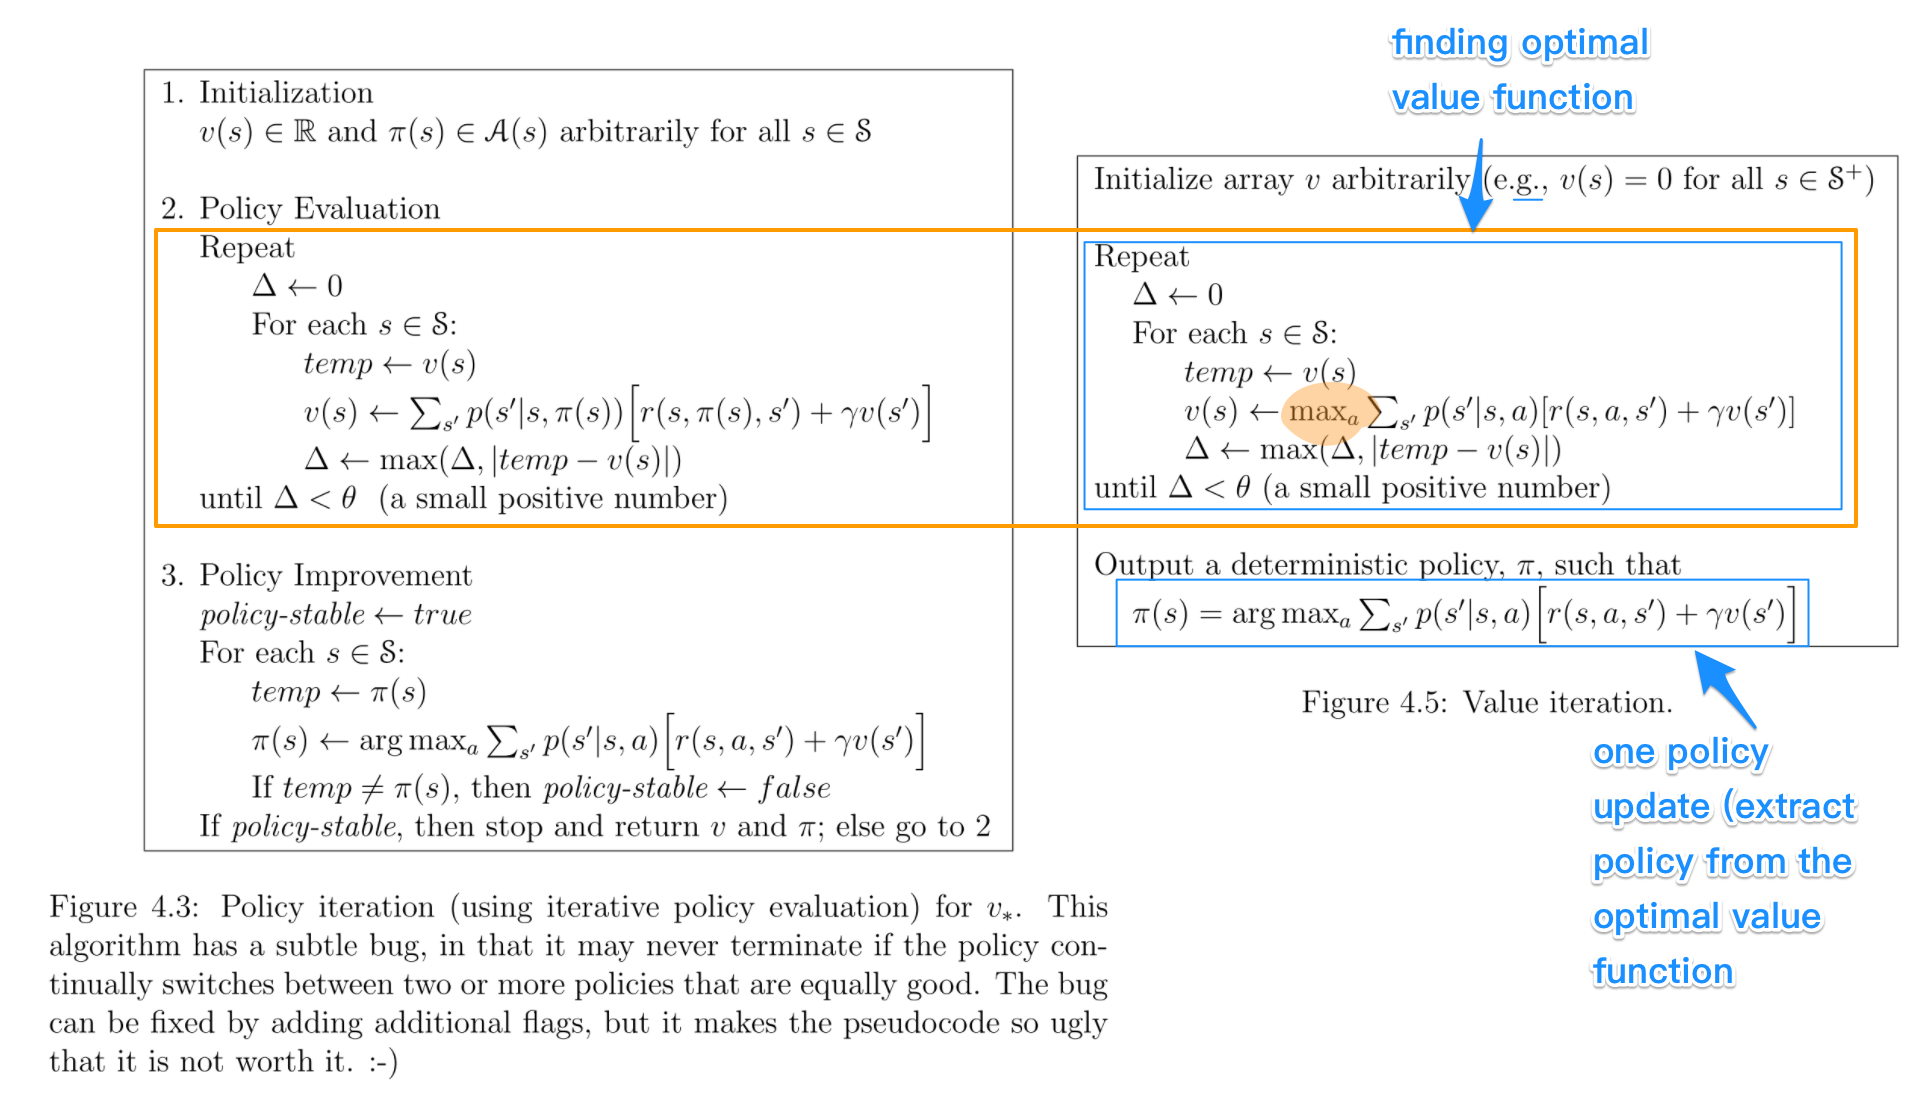
\includegraphics[width=\linewidth]{valueIteration2}
				\end{figure}
				
				\begin{lstlisting}
	import numpy as np
	from gridworld import GridworldEnv

	env = GridworldEnv()
	 
	def value_iteration(env, theta=0.0001, discount_factor=1.0):
	    def one_step_lookahead(state, V):
	        A = np.zeros(env.nA)
	        for a in range(env.nA):
	            for prob, next_state, reward, done in env.P[state][a]:
	                A[a] += prob * (reward + discount_factor * V[next_state])
	        return A
	     
	    V = np.zeros(env.nS)
	    while True:
	        # Stopping condition
	        delta = 0
	        # Update each state...
	        for s in range(env.nS):
	            # Do a one-step lookahead to find the best action
	            A = one_step_lookahead(s, V)
	            best_action_value = np.max(A)
	            # Calculate delta across all states seen so far
	            delta = max(delta, np.abs(best_action_value - V[s]))
	            # Update the value function
	            V[s] = best_action_value        
	        # Check if we can stop 
	        if delta < theta:
	            break
	     
	    # Create a deterministic policy using the optimal value function
	    policy = np.zeros([env.nS, env.nA])
	    for s in range(env.nS):
	        # One step lookahead to find the best action for this state
	        A = one_step_lookahead(s, V)
	        best_action = np.argmax(A)
	        # Always take the best action
	        policy[s, best_action] = 1.0
	     
	    return policy, V
	 
	policy, v = value_iteration(env)
	 
	print("Policy Probability Distribution:")
	print(policy)
	print("")
	 
	print("Reshaped Grid Policy (0=up, 1=right, 2=down, 3=left):")
	print(np.reshape(np.argmax(policy, axis=1), env.shape))
	print("")				
				\end{lstlisting}
		
		
	\section{Model-Free 蒙特卡洛}
		蒙特卡罗强化学习算法通过考虑\textbf{采样轨迹}克服了模型未知给策略估计造成的困难.
		
		多次"\textbf{采样}",然后\textbf{求取平均累积奖赏}来作为期望累积奖赏的近似,这称为蒙特卡罗强化学习.
		
		利用$\epsilon$ 因子,当随机数大于$\epsilon$ 利用,当随机数小于$\epsilon$ 进行探索。换句话说,就是以$1-\epsilon$概率进行利用,以$\epsilon$ 概率进行均匀探索。 
		
		
		
	\section{瞬时差分法: Temporal-Difference TD}
		时序差分(Temporal Difference ,简称 TD) 学习则结合了动态规划与蒙特卡罗方法的思想,能做到更高效的免模型学习.

	\section{Saras}
		在蒙特卡洛的基础上,结合动态规划进行性能提升,使得可以在每一步采样后都可以对Policy 进行提升,采样的策略与提升的策略相同:OnPolicy.
		
		\subsection{Saras}
			单步安全迭代更新
		
		\subsection{Saras($\lambda$)}
			$\lambda$ 步迭代更新。
				
	\section{Q-Learning}
		采样的策略与提升的策略不相同:OffPolicy.
	
		\begin{figure}[H]
			\centering
			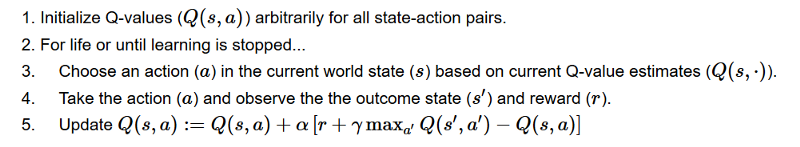
\includegraphics[width=\linewidth]{qFuncProcess2}
			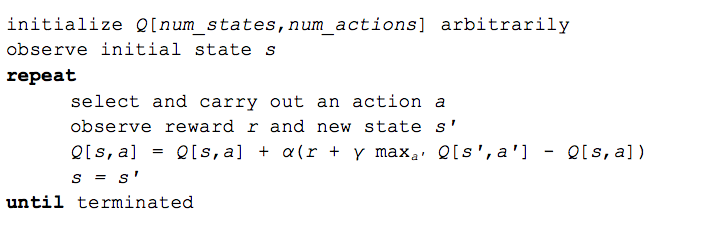
\includegraphics[width=\linewidth]{qFuncProcess3}
		\end{figure}
		\subsection{Q-learning 从案例到原理}	
			\url{http://www.sohu.com/a/228536039_129720}
			
			\paragraph{Environment: Game}
				\textit{the Knight and the Princess}
				
				\begin{figure}[H]
					\centering
					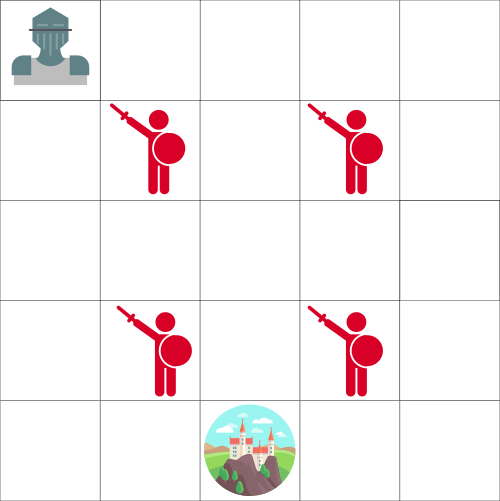
\includegraphics[width=.5\linewidth]{game01}
				\end{figure}
				
				你每次可以移动一个方块的距离。敌人是不能移动的,但是如果你和敌人落在了同一个方块中,你就会死。你的目标是以尽可能快的路线走到城堡去。这可以使用一个「按步积分」系统来评估。
				
				\begin{itemize}
					\item 你在每一步都会失去 1 分, rewardx = -1;
					\item 如果碰到了一个敌人,你会失去 100 分,并且训练 episode 结束。 rewardEnemy = -100;
					\item 如果进入到城堡中,你就获胜了,获得 100 分。 rewardPrincess = 100;
				\end{itemize}
				
				
			\paragraph{Q-table:MDP}
				\subparagraph{Policy $\pi_1$}
					第一个策略。假设智能体试图走遍每一个方块,并且将其着色。绿色代表\textbf{「安全」},红色代表\textbf{「不安全」}。
					
					\begin{figure}[H]
						\centering
						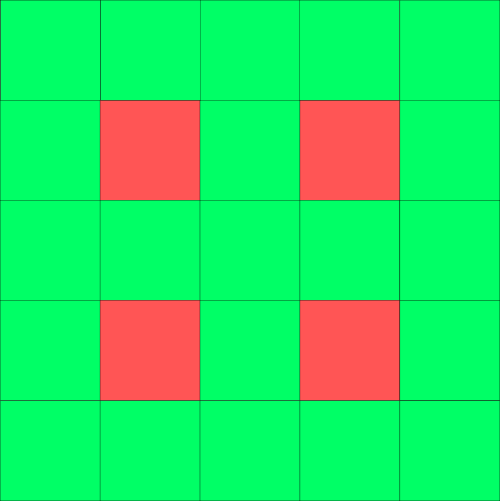
\includegraphics[width=.5\linewidth]{policy01}
					\end{figure}
					
					同样的地图,但是被着色了,用于显示哪些方块是可以被安全访问的。接着,我们告诉智能体只能选择绿色的方块。
					
					但问题是,这种策略并不是十分有用。当绿色的方块彼此相邻时,我们不知道选择哪个方块是最好的。所以,Agent\textit{可能会在寻找城堡的过程中陷入无限的循环}。
					
					
				\subparagraph{Policy $\pi_2$}
					第二种策略:创建一个表格。通过它,我们可以为每一个\textbf{状态(state)}上进行的每一个\textbf{动作(action)}计算出最大的未来\textbf{奖励(reward)的期望}。
					
					得益于这个表格,我们可以知道为每一个状态采取的最佳动作。
					
					每个状态(方块)允许四种可能的操作:左移、右移、上移、下移。
					\begin{figure}[H]
						\centering
						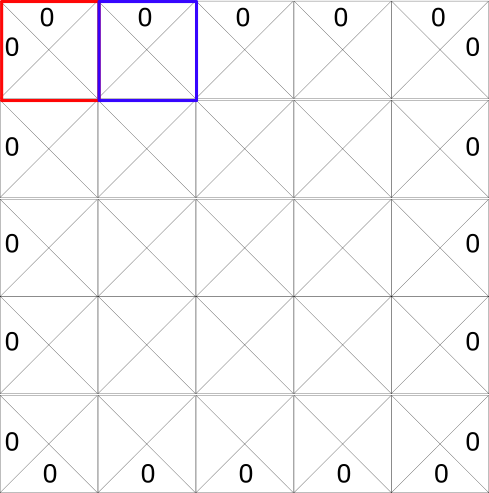
\includegraphics[width=.5\linewidth]{policy02}
					\end{figure}					
					
					
					\textit{「0」代表不可能的移动}(如果你在左上角,你不可能向左移动或者向上移动!)
					
					在计算过程中,我们可以将这个网格转换成一个表。\textbf{这种表格被称为 Q-table(「Q」代表动作的「未来价值」)}。每一列将代表四个操作(左、右、上、下),行代表状态。每个单元格的值代表给定状态和相应动作的最大未来奖励期望。
					\begin{figure}[H]
						\centering
						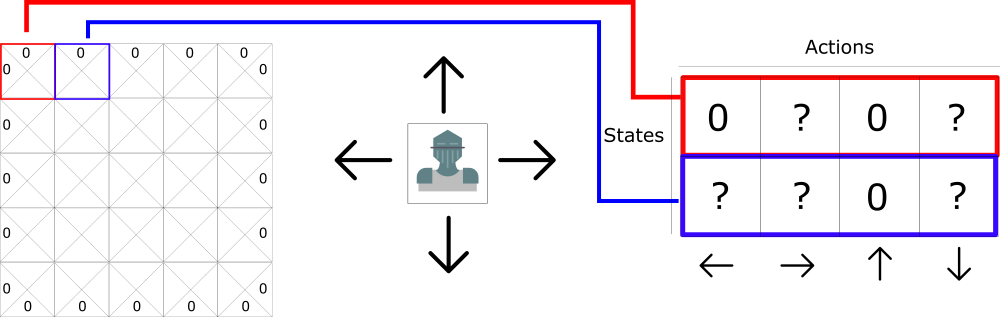
\includegraphics[width=.9\linewidth]{policy02_1}
					\end{figure}
					
					将这个 Q-table 想象成一个「备忘纸条」游戏。得益于此,我们通过寻找每一行中最高的分数,可以知道对于每一个状态(Q-table 中的每一行)来说,可采取的最佳动作是什么。
					这样就解决了这个城堡问题!但是,如何计算 Q-table 中每个元素的值呢?也就是MDP 中提到的BellManEquation。
										
			\paragraph{BellMan-Equation}
				为了求出 Q-table 中的每个值,\textbf{将使用 Q-learning 算法}求解 BellMan Equation. 
				
				\subparagraph{Q-learning 算法:学习动作值函数}
					\textit{动作-值函数}(或称\textit{「Q 函数」})有两个输入:\textbf{「状态」}和\textbf{「动作」}。它将返回\textbf{在该状态下执行该动作的未来奖励期望}。
					
					\begin{figure}[H]
						\centering
						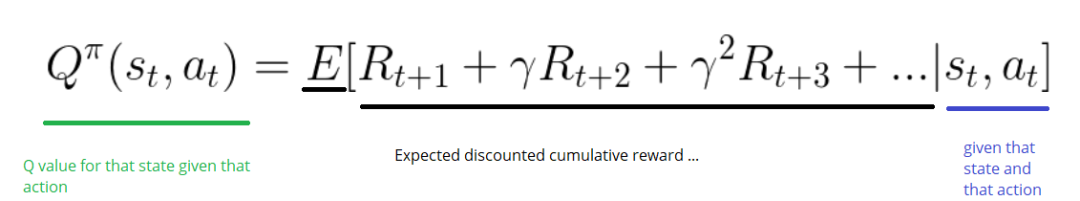
\includegraphics[width=\linewidth]{qFunc}
					\end{figure}
					
					可以把 Q 函数视为一个在 Q-table 上滚动的读取器,用于寻找与当前状态关联的行以及与动作关联的列。\textbf{它会从相匹配的单元格中返回 Q 值。这就是未来奖励的期望}。
					
					在\textbf{探索环境(environment)之前},Q-table 会给出相同的任意的设定值(大多数情况下是 0)。\textbf{随着对环境的持续探索},这个 Q-table 会通过迭代地\textbf{使用 Bellman 方程(动态规划方程)更新 Q(s,a) 来给出越来越好的近似}。具体求解参考动态规范方法一节。
					
				\subparagraph{Q-learning 流程}
					一般计算机模拟流程大概如下:
					
					\begin{figure}[H]
						\centering
						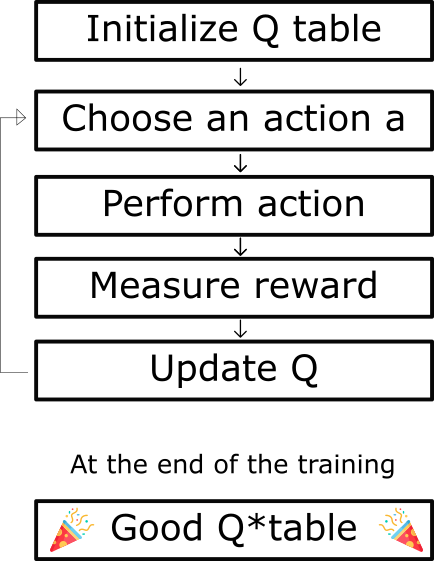
\includegraphics[width=.4\linewidth]{qFuncProcess}
					\end{figure}
				
				
					\begin{itemize}
						\item \textbf{Step 1: Initialize Q-values}
						
							初始化 Q 值。我们构造了一个\textit{ m 列(m = 动作数 ),n 行(n = 状态数)}的 Q-table,并将其中的值\textbf{初始化为 0}。
							
							\begin{figure}[H]
								\centering
								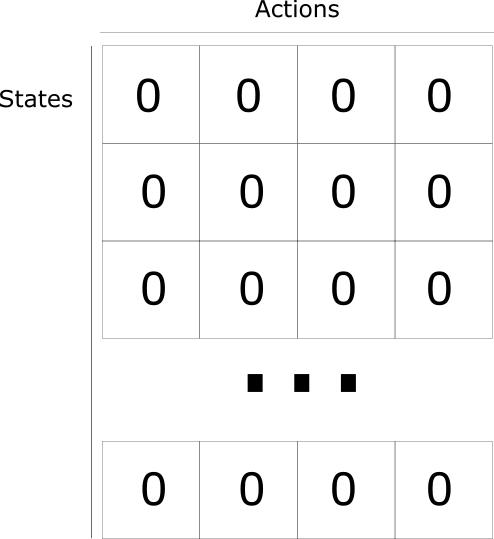
\includegraphics[width=.4\linewidth]{qFuncProcess01}
							\end{figure}
							
						\item \textbf{Step 2: For life (or until learning is stopped)}
							
							在整个生命周期中(或者直到训练被中止前),步骤 3 到步骤 5 会一直被重复,直到达到了最大的训练次数(由用户指定)或者手动中止训练。
							
						\item \textbf{Step 3: Choose an action}
						
							选取一个动作。在基于当前的 Q 值估计得出的状态 s 下选择一个动作 a。
							
							但是……如果每个 Q 值都等于零,我们一开始该选择什么动作呢? 请转到\textbf{$\epsilon$ epsilon 探索/利用 比率} 小节。
						
						\item \textbf{Step 4–5: Evaluate!}
						
							评价!采用动作 a 并且观察输出的状态 s' 和奖励 r。现在我们更新函数 Q(s,a)。
							
							我们采用在步骤 3 中选择的动作 a,然后执行这个动作会返回一个新的状态 s' 和奖励 r。接着我们使用 Bellman 方程去更新 Q(s,a):
							\begin{figure}[H]
								\centering
								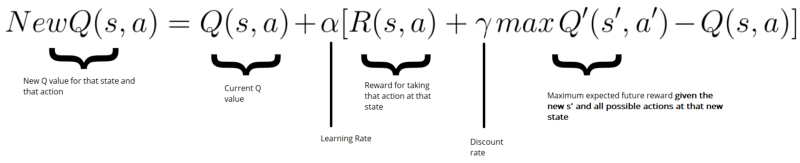
\includegraphics[width=.9\linewidth]{qFuncProcess02}
							\end{figure}	
							
							\begin{lstlisting}
New Q value = Current Q value + lr * [Reward + discount_rate * (highest Q value between possible actions from the new state s’ ) — Current Q value]							
							\end{lstlisting}						
							
					\end{itemize}
				
			
			\paragraph{$\alpha$ 学习率}
				可以将学习率看作是网络\textbf{有多快地抛弃旧值、生成新值的度量}。如果学习率是 1,新的估计值会成为新的 Q 值,并完全抛弃旧值。
			
			\paragraph{$\epsilon$ epsilon 探索/利用 比率}
				在刚开始初始化后,每个 Q 值都等于零,一开始该选择什么动作呢?在这里,就可以看到\textbf{探索/利用}\textbf{(exploration/exploitation)}的权衡有多重要了。
			
				思路就是,在一开始,将使用 \textbf{epsilon 贪婪策略}:
				
				\begin{enumerate}[itemindent = 1em]
					\item 指定一个\textbf{探索速率「epsilon」},一开始将它设定为 1。这个就是我们将随机采用的步长。在一开始,这个速率应该处于最大值,因为我们不知道 Q-table 中任何的值。这意味着,我们需要通过随机选择动作进行大量的探索。
					\item \textit{生成一个随机数}。如果\textbf{这个数大于 epsilon,那么我们将会进行「利用」}(这意味着我们在每一步利用已经知道的信息选择动作)。否则,我们将继续进行探索。
					\item 在刚开始训练 Q 函数时,我们必须有一个大的 epsilon。随着智能体对估算出的 Q 值更有把握,我们将逐渐减小 epsilon。
				\end{enumerate}
				
				\begin{figure}[H]
					\centering
					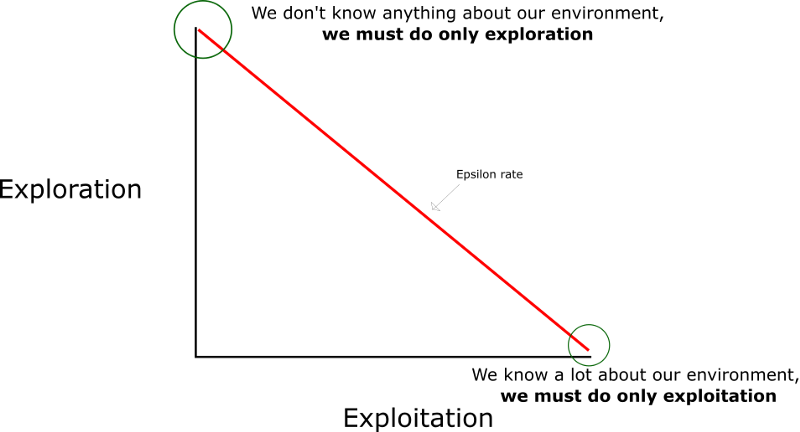
\includegraphics[width=\linewidth]{epsilon}
				\end{figure}
	
	
		\subsection{Q-learning 案例示例}
		
			\paragraph{Environment}
				老鼠奶酪游戏。
				
				\begin{figure}[H]
					\centering
					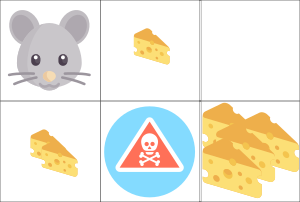
\includegraphics[width=.4\linewidth]{qExample}
				\end{figure}
			
				\begin{itemize}
					\item 一块奶酪 = +1
					\item 两块奶酪 = +2
					\item 一大堆奶酪 = +10(训练结束)
					\item 吃到了鼠药 = -10(训练结束)
				\end{itemize}
			
			
			\paragraph{Step1:初始化 Q-table}
				初始化
				
				\begin{figure}[H]
					\centering
					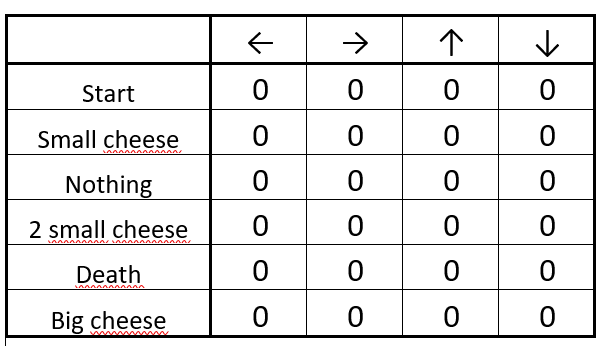
\includegraphics[width=.7\linewidth]{qExample01}
				\end{figure}
			
			\paragraph{Step2、3:选择一个动作}
				从起始点,你可以在向右走和向下走其中选择一个。由于有一个\textbf{大的 epsilon 速率}(因为我们至今对于环境一无所知),我们随机地选择一个。例如向右走。
				\begin{figure}[H]
					\centering
					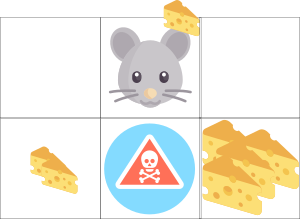
\includegraphics[width=.4\linewidth]{qExample02}
					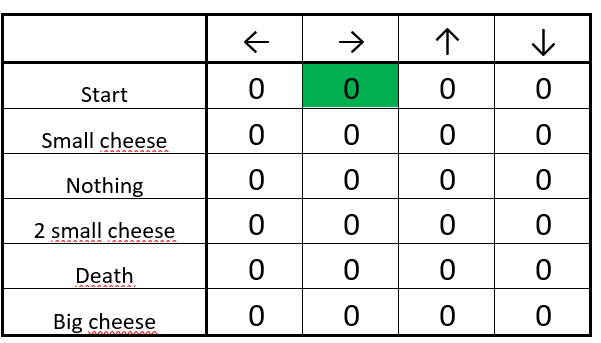
\includegraphics[width=.7\linewidth]{qExample03}
				\end{figure}			
				
				我们随机移动(例如向右走)
				
				我们发现了一块奶酪(+1),现在我们可以更新开始时的 Q 值并且向右走,通过 Bellman 方程实现。
				
			\paragraph{Step4、5:更新Q 函数}
				更新 Q 函数
				\begin{figure}[H]
					\centering
					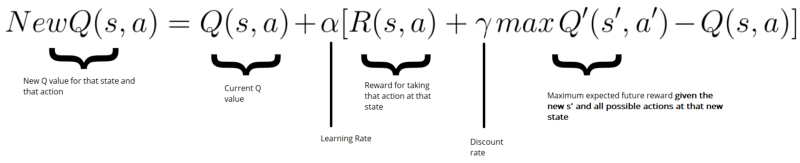
\includegraphics[width=.95\linewidth]{qExample04}
					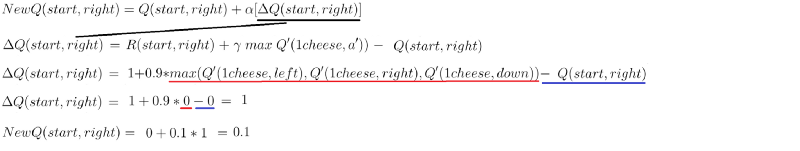
\includegraphics[width=.96\linewidth]{qExample05}
				\end{figure}					
				
				\begin{itemize}
					\item 首先,我们计算 Q 值的改变量$\Delta Q(start, right)$。
					\item 接着我们将初始的 Q 值与$\Delta Q(start, right)$和学习率$\alpha$的积相加。
				\end{itemize}
				
				\begin{figure}[H]
					\centering
					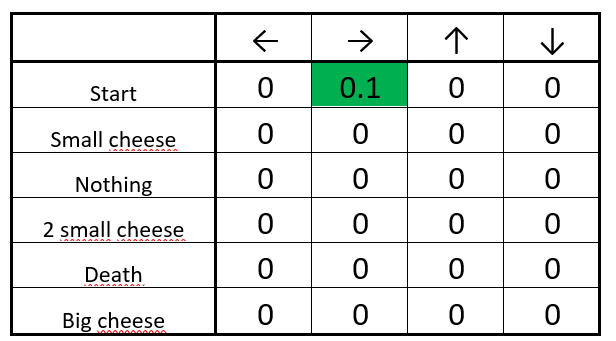
\includegraphics[width=.7\linewidth]{qExample06}
				\end{figure}
				
				刚刚更新了第一个 Q 值。现在我们要做的就是\textbf{一次又一次地做这个工作直到学习结束}。		
		

	
	\section{Deep-Q-Network}
		\url{https://www.jianshu.com/p/41659ce20f15}
	
		这是一种融合了\textbf{神经网络}和 \textbf{Q learning} 的方法, 名字叫做 Deep Q Network.
			\begin{figure}[H]
				\centering
				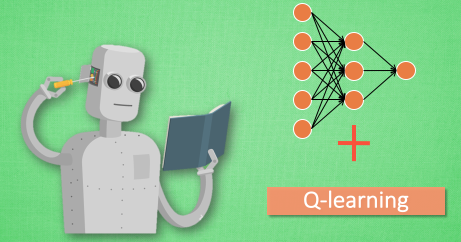
\includegraphics[width=.9\linewidth]{DQN1}
			\end{figure}
			
			\begin{figure}[H]
				\centering
				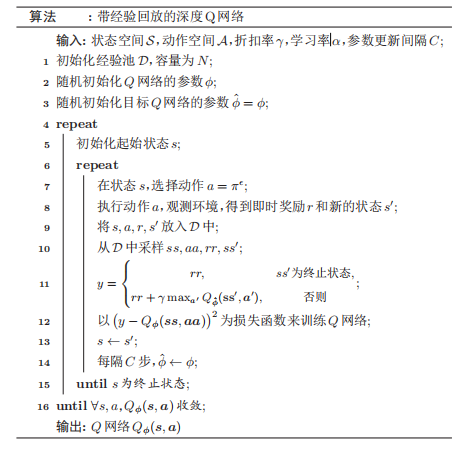
\includegraphics[width=.9\linewidth]{DQN6}
				\caption{DQN 算法概述}
			\end{figure}			
			\begin{figure}[H]
				\centering
				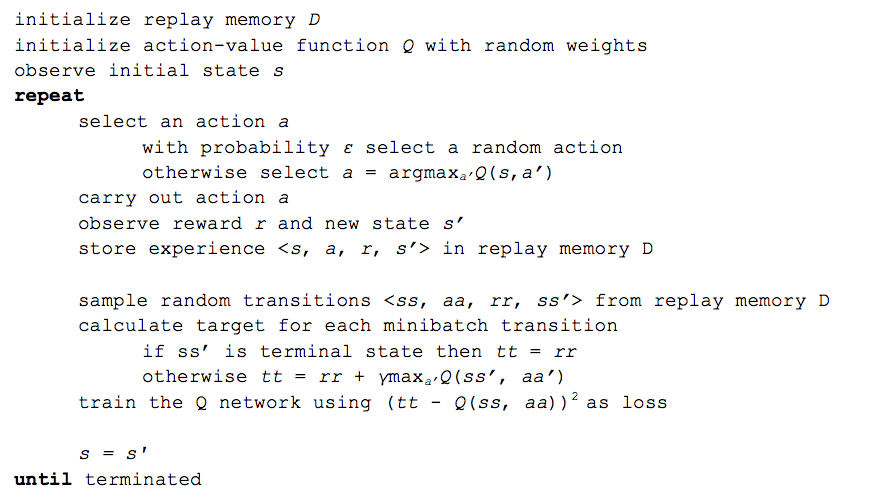
\includegraphics[width=.9\linewidth]{DQN5}
				\caption{DQN 算法概述}
			\end{figure}
		
		\subsection{神经网络的作用}
			使用表格来存储每一个状态 state, 和在这个 state 每个行为 action 所拥有的 Q 值. \textbf{而当今问题是在太复杂, 状态可以多到比天上的星星还多(比如下围棋). 如果全用表格来存储它们, 恐怕我们的计算机有再大的内存都不够, 而且每次在这么大的表格中搜索对应的状态也是一件很耗时的事}. 不过, 在机器学习中, 有一种方法对这种事情很在行, 那就是神经网络. 我们\textbf{可以将状态和动作当成神经网络的输入, 然后经过神经网络分析后得到动作的 Q 值, 这样我们就没必要在表格中记录 Q 值, 而是直接使用神经网络生成 Q 值}. 还有一种形式的是这样, 我们\textbf{也能只输入状态值, 输出所有的动作值, 然后按照 Q learning 的原则, 直接选择拥有最大值的动作当做下一步要做的动作}. 
			
			\begin{figure}[H]
				\centering
				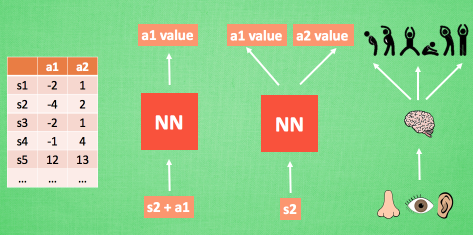
\includegraphics[width=.9\linewidth]{DQN2}
			\end{figure}
		
			我们可以想象, 神经网络接受外部的信息, 相当于眼睛鼻子耳朵收集信息, 然后通过大脑加工输出每种动作的值, 最后通过强化学习的方式选择动作.
			
		\subsection{训练神经网络}
			基于第二种神经网络来分析
			
			我们知道, 神经网络是要被训练才能预测出准确的值. 那在强化学习中, 神经网络是如何被训练的呢? 首先, 我们需要 a1, a2 正确的Q值, 这个 Q 值我们就用之前在 Q learning 中的 Q 现实来代替. 同样我们还需要一个 Q 估计 来实现神经网络的更新. 所以神经网络的的参数就是老的 NN 参数 加学习率 alpha 乘以 Q 现实 和 Q 估计 的差距. 我们整理一下.
			\begin{figure}[H]
				\centering
				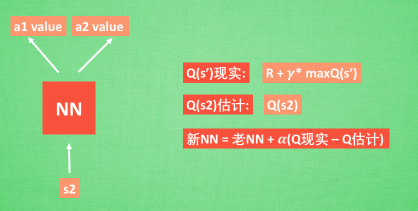
\includegraphics[width=.9\linewidth]{DQN3}
				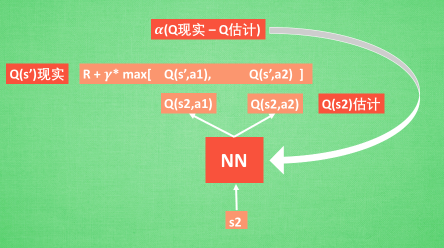
\includegraphics[width=.9\linewidth]{DQN4}
			\end{figure}			
			通过 NN 预测出Q(s2, a1) 和 Q(s2,a2) 的值, 这就是 Q 估计. 然后我们选取 Q 估计中最大值的动作来换取环境中的奖励 reward. 而 Q 现实中也包含从神经网络分析出来的两个 Q 估计值, 不过这个 Q 估计是针对于下一步在 s’ 的估计. 最后再通过刚刚所说的算法更新神经网络中的参数. 但是这并不是 DQN 会玩电动的根本原因. 还有两大因素支撑着 DQN 使得它变得无比强大. 这两大因素就是 Experience replay 和 Fixed Q-targets.
		
		\subsection{经验回放}
			\textit{构建一个经验池(Replay Buffer)来去除数据相关性。经验池是由智能体最近的经历组成的数据集。}
		
			事实证明,使用非线性函数得到近似的 Q 值是不稳定的。要使它真正收敛还需要加入很多技巧,而且要花费很长的时间,即使使用一个 GPU 也要耗上差不多一周的时间。
			
			最重要的一个技巧就是经验回放。在游戏过程中,所有的经历 <s, a, r, s'> 都存储在一个可回顾的记忆模块中。训练神经网络的时候,会从记忆中取出随机小批量的记忆片段来训练,而不是直接使用最近期的经历。这样就切断了之后相似训练情况的连续性,这种相似性往往会使整个网络局限于一小块状态区域。此外,经验回放使训练任务更类似于通常的监督学习,这简化了调试和测试算法。而且也可以直接收集人类玩游戏的经验,在此基础上继续训练。
		
		\subsection{目标网络冻结}
			\textit{目标网络冻结(Freezing Target Networks),即在一个时间段内固定目标中的参数,来稳定学习目标}
		
		\subsection{DQN 两大利器}
			DQN 有一个记忆库用于学习之前的经历, Q learning 是一种 off-policy 离线学习法, 它能学习当前经历着的, 也能学习过去经历过的, 甚至是学习别人的经历. 所以每次 DQN 更新的时候, 我们都可以随机抽取一些之前的经历进行学习. 随机抽取这种做法打乱了经历之间的相关性, 也使得神经网络更新更有效率. 
			
			Fixed Q-targets 也是一种打乱相关性的机理, 如果使用 fixed Q-targets, 我们就会在 DQN 中使用到两个结构相同但参数不同的神经网络, 预测 Q 估计 的神经网络具备最新的参数, 而预测 Q 现实 的神经网络使用的参数则是很久以前的. 
	
	
	\section{Policy Gradient}
		\url{https://www.jianshu.com/p/2ccbab48414b}
		
		\subsection{ReinForce 算法}
			策略梯度的基本思想,就是直接根据状态输出动作或者动作的概率。
			
			在训练神经网络中,使用最多的方法就是反向传播算法,其中需要一个误差函数,通过梯度下降来使损失函数的值最小化。但对于强化学习来说,我们不知道动作的正确与否,只能通过奖励值来判断这个动作的相对好坏。基于上面的想法,有个非常简单的想法:
			
			\textbf{如果一个动作得到的reward多,那么我们就使其出现的概率增加,如果一个动作得到的reward少,我们就使其出现的概率减小。}
			
			根据这个思想,可以构造如下的损失函数:$loss= -log(prob)*vt$
			
			\begin{itemize}
				\item $log(prob)$ 表示在状态 s 对所选动作 a 的\textbf{吃惊度}, \textit{如果概率越小, 反向的log(prob) 反而越大}
				\item $vt$ 代表的是当前状态s下采取动作a所能得到的奖励,这是当前的奖励和未来奖励的贴现值的求和
			\end{itemize}
		
			也就是说,我们的策略梯度算法\textbf{必须要完成一个完整的eposide}才可以进行参数更新,而不是像值方法那样,每一个$(s,a,r,s')$都可以进行参数更新。
			
			Policy Gradient的核心思想是更新参数时有两个考虑:如果这个回合选择某一动作,下一回合选择该动作的概率大一些,然后再看奖惩值,如果奖惩是正的,那么会放大这个动作的概率,如果奖惩是负的,就会减小该动作的概率。
			
			策略梯度的过程如下图所示:
			\begin{figure}[H]
				\centering
				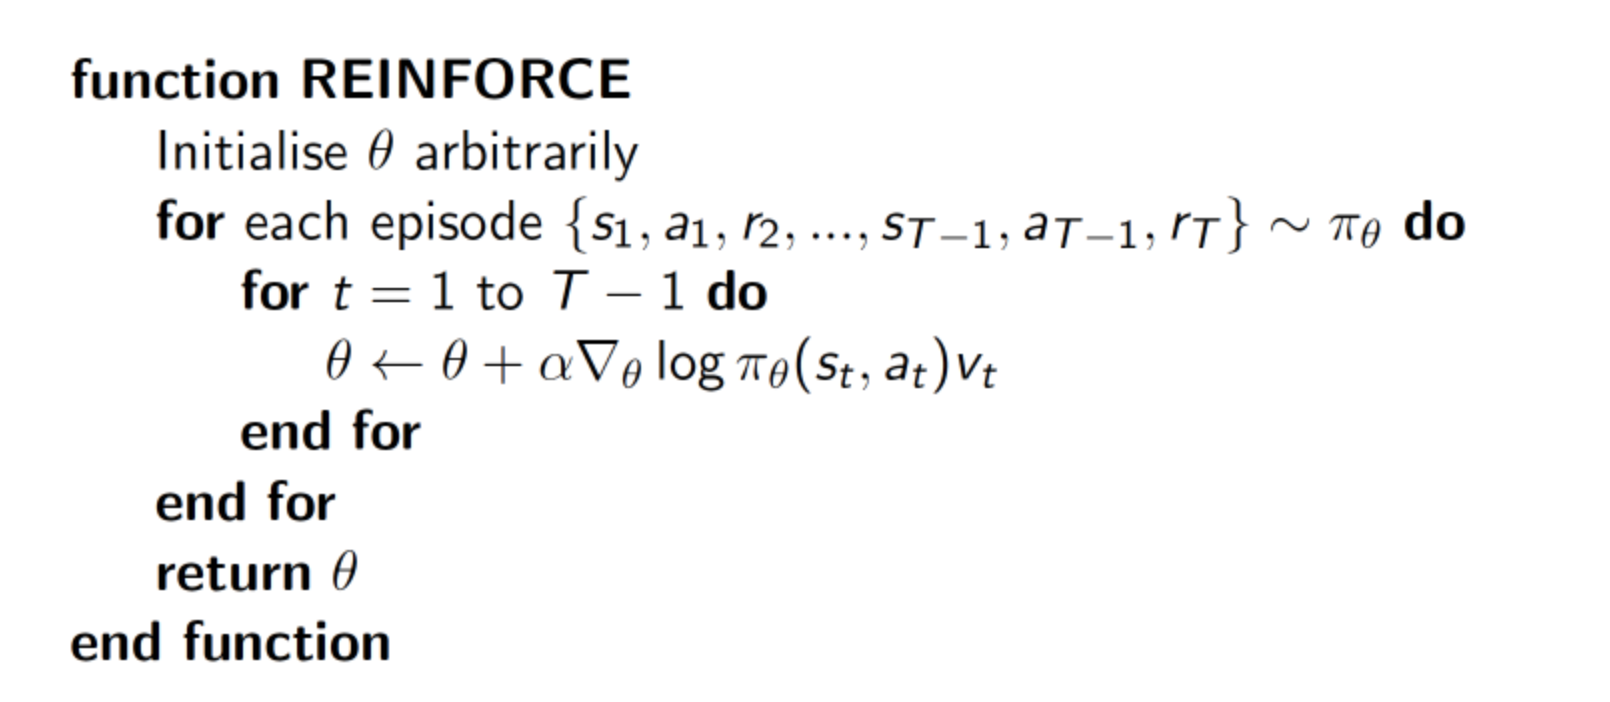
\includegraphics[width=.8\linewidth]{PolicyGradient}
				\caption{策略梯度}
			\end{figure}
			
			最后再强调Policy Gradient的一些细节:
			\begin{itemize}
				\item 算法输出的是\textbf{动作的概率},而不是Q值。
				\item 损失函数的形式为:$loss= -log(prob)*vt$
				\item \textbf{需要}一次\textbf{完整的episode}才可以进行参数的更新
			\end{itemize}
		
		\subsection{带基准线的 ReInforce 算法}
			REINFORCE 算法的一个主要缺点是不同路径之间的方差很大,导致训练不稳定,这是在高维空间中使用蒙特卡罗方法的通病。一种减少方差的通用方法是引入一个控制变量。
			
			假设要估计函数f 的期望,为了减少f 的方差,我们引入一个已知期望的函数g,令
			
			$$\hat{f} = f - \alpha(g - E[g]).$$
			
			因为$E[\hat{f}] = E[f]$,我们可以用$\hat{f}$ 的期望来估计函数f 的期望,同时利用函数g 来减小 $\hat{f}$ 的方差。
			
	\section{Actor-Critic}
		实现:\url{https://blog.csdn.net/qq_30615903/article/details/80774384}
		
		理论:\url{https://zhuanlan.zhihu.com/p/36494307}
		
		
		Actor-Critic算法分为两部分,我们分开来看actor的前身是policy gradient他可以轻松地在连续动作空间内选择合适的动作,value-based的Qlearning做这件事就会因为空间过大而爆炸,但是又因为Actor是基于回合更新的所以学习效率比较慢,这时候我们发现可以使用一个value-based的算法作为Critic就可以实现单步更新。这样两种算法相互补充就形成了我们的Actor-Critic.

		\begin{figure}[H]
			\centering
			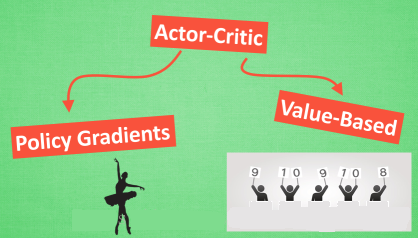
\includegraphics[width=.9\linewidth]{Actor-Critic}
		\end{figure}
		
		\textbf{Actor 基于概率选行为, Critic 基于 Actor 的行为评判行为的得分, Actor 根据 Critic 的评分修改选行为的概率。}
		
		
	\section{模仿学习}
		在强化学习的经典任务设置中,机器所能获得的反馈信息仅有多步决策后的累积奖赏,但在现实任务中,往往能得到人类专家的决策过程范例,例如在种瓜任务上能得到农业专家的种植过程范例.从这样的范例中学习,称为"模仿学习" (imitation "learning).	
		
		强化学习任务中多步决策的搜索空间巨大,基于累积奖赏来学习很多步之前的合适决策非常困难'而直接模仿仿,人类专家的"状态-动作对 白闯民显显著缓解这一困难'我们称其为"直接模仿学习。
		
		
				
\chapter{统计数学方法-李航}


\chapter{神经网络与机器学习-SimonHaykn}
	\section{什么是神经网络}
		\begin{figure}[H]
			\centering
			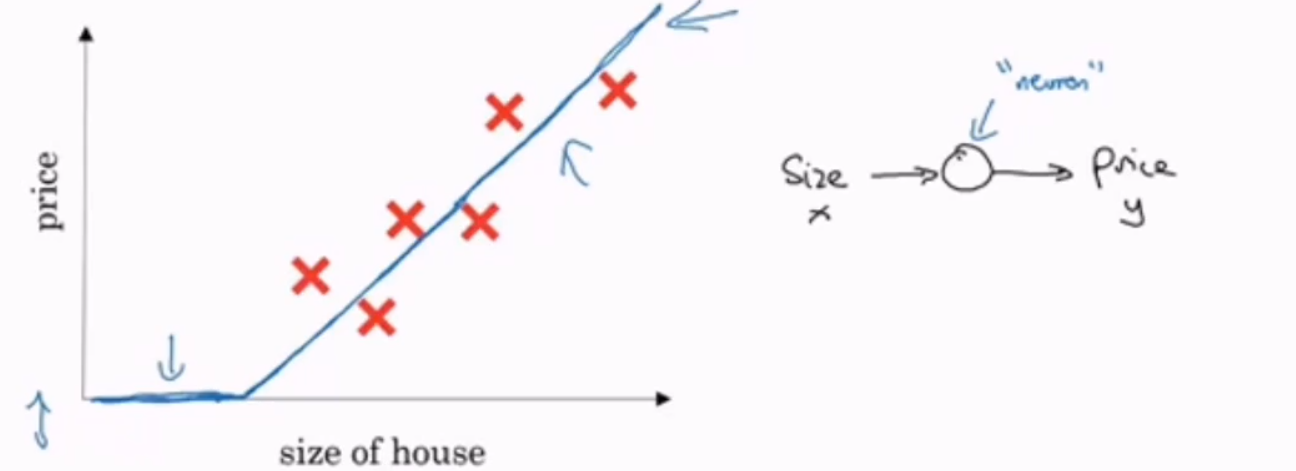
\includegraphics[width=\linewidth]{Neuron}
			\caption{单神经元}
		\end{figure}
	
	
		\begin{figure}[H]
			\centering
			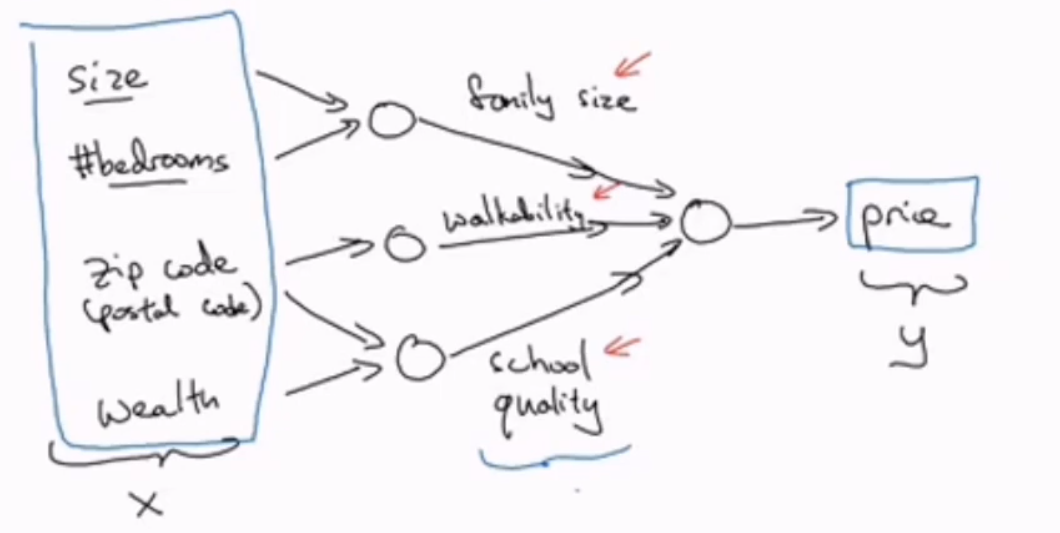
\includegraphics[width=\linewidth]{Neuron2}
			\caption{神经网络}
		\end{figure}
	
	

\chapter{机器学习-周志华、吴恩达}


\chapter{深度学习-花书}

\chapter{贯通-OReilly.Hands-On.Machine.Learning}


\chapter{案例分析}


\chapter{应用}



  
		    
\end{document} 
 		    